% Compile from this directory: tectonic --keep-logs Problem4_Chinese_Tutorial.tex
\documentclass[11pt,a4paper,fontset=none]{ctexart}
\usepackage[margin=24mm,headheight=15pt]{geometry}
\usepackage{fontspec}
\setCJKmainfont{Noto Serif CJK SC}[BoldFont={Noto Serif CJK SC Bold}]
\setCJKsansfont{Noto Sans CJK SC}
\setCJKmonofont{Noto Sans Mono CJK SC}
\usepackage{amsmath,amssymb,mathtools,booktabs,tabularx,longtable,array}
\usepackage{graphicx,float,caption,xcolor,listings,enumitem,fancyhdr}
\usepackage{etoolbox}
\usepackage[unicode,colorlinks=true,linkcolor=blue!45!black,urlcolor=blue!55!black,citecolor=blue!45!black]{hyperref}
\usepackage{bookmark}
\definecolor{ink}{HTML}{203649}
\definecolor{accent}{HTML}{236C86}
\definecolor{papergray}{HTML}{F4F6F8}
\ctexset{section={format=\Large\bfseries\sffamily\color{ink}},subsection={format=\large\bfseries\sffamily\color{ink}}}
\linespread{1.22}
\setlength{\parskip}{3pt}
\setlength{\emergencystretch}{3em}
\setlist{itemsep=3pt,topsep=5pt,parsep=1pt}
\captionsetup{font=small,labelfont=bf,skip=7pt}
\setcounter{tocdepth}{2}
\numberwithin{equation}{section}
\newcommand{\E}{\mathbb E}
\newcolumntype{Y}{>{\raggedright\arraybackslash}X}
\DeclareMathOperator{\Var}{Var}
\DeclareMathOperator{\Cov}{Cov}
\newcommand{\R}{\mathbb R}
\lstset{language=Python,basicstyle=\ttfamily\footnotesize,keywordstyle=\color{blue!65!black},
  commentstyle=\color{green!35!black},stringstyle=\color{orange!60!black},
  numbers=left,numberstyle=\tiny\color{gray},numbersep=6pt,
  showstringspaces=false,breaklines=true,breakatwhitespace=false,
  frame=single,rulecolor=\color{black!15},backgroundcolor=\color{papergray},
  columns=fullflexible,keepspaces=true,tabsize=4,xleftmargin=1.2em,framexleftmargin=.5em}
\pagestyle{fancy}
\fancyhf{}
\fancyhead[L]{\small 第四题中文学习讲义}
\fancyhead[R]{\small 概率论基础 → 随机微分方程 → 数值实验}
\fancyfoot[C]{\thepage}
\renewcommand{\headrulewidth}{.3pt}
\pretocmd{\section}{\clearpage}{}{}
\hypersetup{pdftitle={第四题：金融随机微分方程——从概率论到代码},pdfauthor={中文学习讲义},pdfsubject={基于现有 Problem 4 文件的中文教学说明}}
\begin{document}
\hypersetup{pageanchor=false}
\begin{titlepage}
\vspace*{20mm}
{\sffamily\color{accent}\large Problem Pack · Direction 4\par}
\vspace{8mm}
{\sffamily\bfseries\Huge 金融随机微分方程\par}
\vspace{5mm}
{\sffamily\LARGE 从概率论基础到理论推导与代码实现\par}
\vspace{12mm}
{\large 基于本文件夹已有报告、Python 源码和数值结果的中文讲义\par}
\vspace{12mm}
\noindent\begin{minipage}{.93\textwidth}
你已经学过随机变量、期望、方差、正态分布与大数定律。这些知识足以开始学习本题。
本讲义先解释“随机驱动的连续时间模型”是什么意思，再推导 Itô 公式、几何布朗运动的精确解和两种数值方法，最后把每个概念落实到现有程序和实验数据。
\end{minipage}
\vfill
\noindent\textbf{阅读对象：}没有随机微积分和随机微分方程基础的学习者。\\[4pt]
\textbf{材料范围：}原题第 6--7 页；现有 GBM 与非仿射波动率两组实验。\\[4pt]
\textbf{版本：}2026 年 9 月 12 日。\\[4pt]
\textbf{配套文件：}\texttt{teaching\_demo.py} 为独立教学示例，原实验数据另行保留。
\end{titlepage}
\pagenumbering{roman}
\hypersetup{pageanchor=true}
\tableofcontents
\clearpage
\pagenumbering{arabic}

\section{先读懂题目：我们究竟要解决什么问题？}\label{sec:question}
\subsection{题目的主线是验证数值方法，而不是预测股价}
原题给出五个研究方向，其中第四个方向讨论金融随机微分方程\cite{pack}。
“随机”意味着：即使初值和参数完全相同，未来仍会因为随机冲击而出现许多不同路径。
因此，输出不是唯一一条确定曲线，而是一组可能的价格路径以及它们的统计规律。
这份作业使用人为规定的参数，不涉及用市场数据估计参数，也没有要求给出买卖建议。

第四题安排了两个层次。第一层是几何布朗运动，简称 GBM，它有精确解。
我们先假装不知道精确解，用数值方法计算，再与精确答案比较，检查方法和程序是否可靠。
第二层是非仿射随机波动率模型，它的波动率本身会随机变化。
原题指出，这个一般模型没有已知的实用精确采样器；我们改用更细的数值网格作为参考，并检查参考自身是否稳定。
它在原题中列为推荐扩展，现有文件已经完成了这一部分，所以本讲义也完整讲解。

这里的“精确模拟”指网格时刻的值服从精确转移规律；在同一个布朗运动驱动下，也能直接给出该时刻的真值。
它不表示计算机储存了连续时间里的无限多个点，更不表示用有限样本估计期望时没有抽样误差。

\subsection{把原题要求翻译成可执行的任务}
表~\ref{tab:tasks} 给出题意、数学量与现有实现的对应。
不要把其他 ODE 方向的 Euler、RK4、隐式方法、稳定域和自适应步长要求照搬过来：
原题开头明确规定，第四题采用 SDE 的专门比较要求。
文件夹里的 \texttt{tutorial1/} 是较早的 ODE 学习材料，其中 RK4 稳定域代码不是本题随机方法的实现。

\begin{table}[htbp]\centering\small
\caption{题目要求与现有文件的对应。}\label{tab:tasks}
\begin{tabularx}{\textwidth}{p{.22\textwidth}YY}\toprule
任务 & 实际要回答的问题 & 主要材料\\\midrule
GBM 精确、EM、Milstein 比较 & 相同随机冲击下，数值终值距离真值有多远？ & \texttt{gbm.py}\\
强收敛 & 步长减半后，平均绝对路径误差如何下降？ & \texttt{gbm\_convergence.csv}\\
弱收敛 & 数值方法造成的均值偏差是否与步长成正比？ & 配对差、控制变量及解析偏差\\
分布验证 & 终值的直方图和分位数是否符合对数正态分布？ & 分布图与分位数表\\
正值性（选做） & 更新公式是否可能把正价格变成负数？ & 更新乘子的理论分析\\
非仿射模型 & 如何同步更新对数价格和随机波动因子？ & \texttt{nonaffine.py}\\
参考网格验证 & 更换更细参考后，结论变化多大？ & 三组参考网格及差异表\\
程序核验 & 增量、状态、统计量和保存数据是否相互一致？ & \texttt{verify.py}、JSON、NPZ\\\bottomrule
\end{tabularx}
\end{table}

\subsection{符号与阅读路线}
一个实验有两个不同的“数量”：每条路径有 $N$ 个时间步，总共模拟 $M$ 条路径。
增加 $N$ 改善时间离散，增加 $M$ 改善统计估计；两者不可混淆。
表~\ref{tab:notation} 是贯穿讲义的符号表。

\begin{table}[htbp]\centering
\caption{主要符号。}\label{tab:notation}
\begin{tabularx}{\textwidth}{lY}\toprule
符号 & 含义\\\midrule
$t,T$ & 当前时刻、终止时刻；本实验 $T=1$\\
$N,h=T/N$ & 一条路径的步数、每一步的时间长度\\
$M,i$ & 独立路径总数、路径编号\\
$n,t_n=nh$ & 时间步编号、网格时刻\\
$W_t,\Delta W_n$ & 布朗运动、$W_{t_{n+1}}-W_{t_n}$\\
$S_t,S_n^{(h)}$ & 连续模型的价格、步长 $h$ 下的数值价格\\
$X_t=\log S_t$ & 对数价格；不是另外一种资产\\
$Y_t,g(Y_t)$ & 波动因子、由波动因子决定的瞬时波动率\\
$\mu,\sigma$ & GBM 的相对漂移率和波动率\\
$\varphi(s)$ & 要比较期望的函数，如 $s$ 或 $\max(s-100,0)$\\
$\E,\Var,\Cov$ & 期望、方差、协方差\\
$\mathcal F_t$ & 到时刻 $t$ 为止可以使用的信息\\\bottomrule
\end{tabularx}
\end{table}

建议按目录顺序学习。控制变量的五个具体公式安排在后面的进阶部分：第一次阅读可先理解“减去一个均值为零、又与误差相关的随机量”，等掌握基本仿真流程后再读完整推导。
讲义中的大型实验数值来自现有保存文件，并非把小规模教学脚本的输出当作原实验结果。
我们对保存数组与统计量进行了独立复核；本次没有重新运行原来的全部大型随机实验。


\section{从概率论走向随机微积分：先补齐语言}
\label{bg:sec:language}

本节先用 $X$ 泛指一般随机过程；进入金融模型后，$S$ 专指价格，$X=\log S$ 专指对数价格。
题目中的 $W_t$、$\mathrm dW_t$ 和 $\mathrm dX_t$ 看起来都带着微积分符号，
但不能直接按普通导数运算。本节从已经熟悉的随机变量出发，说明这些符号究竟代表什么。
学习时先抓住三个问题：\emph{随机性在哪里？在时刻 $t$ 已经知道什么？一个很短时间段中的变化有多大？}
这三个问题贯穿后面的公式推导和程序实现。

\subsection{随机变量是一张照片，随机过程是一段随机影片}
\label{bg:sub:process}

一个随机变量 $Y$ 给每个可能的实验结果 $\omega$ 指定一个数 $Y(\omega)$。
随机过程则是一族带时间下标的随机变量 $\{X_t:t\geq 0\}$。
这里有两种不同的观察方式：固定时间 $t$，$X_t$ 是一个随机变量，可以讨论其均值、方差和分布；
固定一次实验结果 $\omega$，映射 $t\mapsto X_t(\omega)$ 是一条\emph{样本路径}。
模拟一次完整实验，得到一条路径；重新抽取随机数，通常会得到另一条路径。

例如，用 $S_t$ 表示时刻 $t$ 的资产价格。$S_1$ 表示一年后的随机价格，
而整条 $\{S_t:0\leq t\leq 1\}$ 还记录这一年中价格经过了哪些位置。
终点分布相同的两个模型，中途波动方式可能很不一样。
这也解释了为什么“比较终点平均价格”和“逐条比较两种模拟得到的路径”是两件不同的事。

在计算机中，连续时间通常被离散成一个网格。若总时长为 $T$，分成 $N$ 步，则
\begin{equation}
  h=\frac{T}{N},\qquad t_n=nh,\qquad n=0,1,\ldots,N.
  \label{bg:eq:grid}
\end{equation}
一条离散路径就是长度为 $N+1$ 的数列 $(X_0,X_1,\ldots,X_N)$，
其中程序中的 $X_n$ 通常代表连续过程在 $t_n$ 附近的近似值。
网格越密意味着时间分辨率越高；增加模拟路径数则是重复更多次随机实验。
这两个操作改变的是不同的量。

还要区分随机变量与随机变量的一次数值实现。表达式 $\E[X_T]$ 是模型分布决定的一个数；
某次模拟的终点 $X_T(\omega)$ 只是一个观测值，不会因为计算正确就恰好等于该均值。
把很多条路径在同一时刻取平均，可以观察平均行为；把同一条路径在很多时刻取平均，
得到的则是另一个统计量。两种平均不能在没有依据时互换。

\subsection{普通微分方程为什么可以改写成积分方程}
\label{bg:sub:ode}

先暂时去掉随机性。普通微分方程
\begin{equation}
  \frac{\mathrm dx(t)}{\mathrm dt}=a(t,x(t)),\qquad x(0)=x_0
  \quad\Longleftrightarrow\quad
  x(t)=x_0+\int_0^t a(s,x(s))\,\mathrm ds
  \label{bg:eq:ode}
\end{equation}
表示当前位置等于初始位置加上从开始到现在的累计变化。
例如 $a(t,x)=rx$ 表示瞬时增长速度与当前数量成正比。
在一个短时间段内把增长速度暂时冻结在左端，就得到
\begin{equation}
  x(t_{n+1})-x(t_n)\approx a(t_n,x(t_n))h.
  \label{bg:eq:ode-euler}
\end{equation}
这是普通 Euler 方法的来源。
随机微分方程也将采用“初值加累计变化”的表达方式，
只是累计变化中多出一种随机积分。因此，理解随机积分比寻找 $W_t$ 的普通导数更重要。

\section{布朗运动：把连续时间的随机冲击建模}
\label{bg:sec:brownian}

\subsection{定义与最需要记住的尺度}
\label{bg:sub:brownian-definition}

标准布朗运动 $W=\{W_t:t\geq0\}$ 满足：$W_0=0$；样本路径几乎必然连续；
不相交时间区间上的增量相互独立；并且对 $0\leq s<t$，
\begin{equation}
  W_t-W_s\sim\mathcal N(0,t-s).
  \label{bg:eq:brownian-increment}
\end{equation}
记号 $\mathcal N(m,v)$ 的第二个参数是\emph{方差}。
特别地，长度为 $h$ 的时间段中的增量可以写成
\begin{equation}
  \Delta W_n=W_{t_{n+1}}-W_{t_n}=\sqrt h\,Z_n,
  \qquad Z_n\sim\mathcal N(0,1),
  \label{bg:eq:normal-scaling}
\end{equation}
其中不同时间段使用独立的 $Z_n$。于是
\begin{equation}
  \E[\Delta W_n]=0,\qquad
  \Var(\Delta W_n)=h,\qquad
  \operatorname{sd}(\Delta W_n)=\sqrt h.
  \label{bg:eq:increment-moments}
\end{equation}

独立的是不相交时间段的\emph{增量}，不是不同时间的布朗运动取值。
例如 $W_t$ 包含此前的 $W_s$，所以它们共享历史波动。对 $s\leq t$，
\begin{equation}
  \Cov(W_s,W_t)=\E[W_s(W_s+W_t-W_s)]=s,
  \label{bg:eq:brownian-covariance}
\end{equation}
其中交叉项因独立且零均值而为零。
如果在每个时间点分别抽取一个独立的 $\mathcal N(0,t)$ 变量，虽然每个时点的边际分布正确，
时间点之间的关系却错了，因而不会得到布朗路径。正确做法是生成独立增量，再累计成取值。

\textbf{随机增量的典型大小是 $\sqrt h$，不是 $h$。}
“典型大小”在这里可由标准差衡量，不能理解为每一次增量都等于 $\sqrt h$。
例如 $h=0.01$ 时，单位布朗运动的增量标准差为 $0.1$。
如果误写成 $hZ_n$，$N=T/h$ 步累计增量的方差将是 $Nh^2=Th$，
随着网格加密趋于零；正确写成 $\sqrt h Z_n$，累计方差则为 $Nh=T$。
前一种写法会在极限中把随机波动抹掉。

比较 $h$ 与 $\sqrt h$ 还有一个容易误解的地方：在足够短的时间段里，
非零扩散项的典型幅度可能比漂移项大，但这不表示漂移在整个时间区间内不重要。
连续 $N$ 步的同向确定性变化按 $Nh$ 累积，独立零均值随机冲击则通过方差按 $Nh$ 累积，
其标准差按 $\sqrt{Nh}$ 衡量。局部尺度的比较与长时间累计效果的比较，需要分别进行。

虽然路径连续，布朗运动却不是一条光滑曲线。
例如在固定时刻观察短区间的差商，有
\begin{equation}
  \frac{W_{t+h}-W_t}{h}\sim\mathcal N\!\left(0,\frac1h\right).
  \label{bg:eq:brownian-difference-quotient}
\end{equation}
它的尺度随 $h\downarrow0$ 而增大，已经提示普通导数的直觉不适用。
更强的结论是布朗样本路径几乎必然处处不可微；这里只把它作为背景事实，
不把差商的分布计算冒充这一结论的完整证明。
因此，$\mathrm dW_t/\mathrm dt$ 不能当作一个普通函数代入常微分方程。

\begin{figure}[htbp]\centering
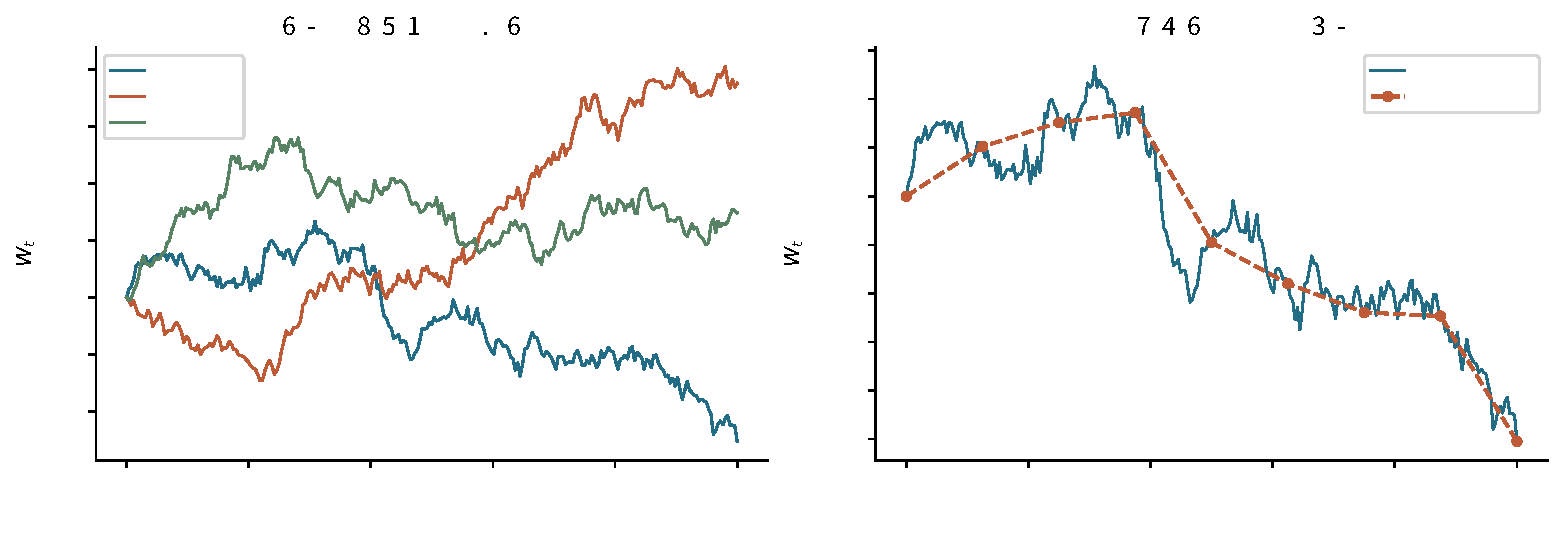
\includegraphics[width=\textwidth]{assets/brownian_coupling.pdf}
\caption{左图展示同一布朗模型的不同样本路径；右图展示同一路径的粗细网格取值。细网格之间也用直线连接以便展示，折线不是连续布朗运动的完整轨迹。}\label{fig:bg-brownian}
\end{figure}
图~\ref{fig:bg-brownian} 右图中，粗网格在共同时间点与细网格完全一致，因为每个粗增量来自相邻细增量求和。后面的强收敛实验正要使用这种设计。

\subsection{用随机游走理解布朗运动的来源}
\label{bg:sub:random-walk}

可以想象每隔 $h$ 秒抛一次公平硬币，向上或向下走 $\sqrt h$：
\begin{equation}
  R_{kh}^{(h)}=\sqrt h\sum_{j=1}^k\xi_j,
  \qquad
  \Pr(\xi_j=1)=\Pr(\xi_j=-1)=\frac12,
  \label{bg:eq:random-walk}
\end{equation}
其中 $\xi_j$ 独立。走过时间 $kh$ 后，均值为零，方差为 $kh$。
当 $h$ 变小，同一段时间内包含越来越多的小冲击。
中心极限定理解释了为什么在固定时间观察时，累计位移接近正态分布；
独立投掷也保留了不相交区间增量的独立性。
进一步的过程极限定理能够把适当插值后的整条随机游走与布朗运动联系起来，
但该结论比单个随机变量的中心极限定理更强，本讲义不证明它。

数值计算不必真的抛硬币。利用式\eqref{bg:eq:normal-scaling}直接生成独立正态增量，
就能\emph{精确生成布朗运动在所选网格上的联合分布}。
这并不意味着已精确得到某个随机微分方程的解；从布朗增量更新状态的公式，仍可能产生离散误差。

\section{信息、条件期望与鞅：为什么不能偷看未来}
\label{bg:sec:information}

\subsection{把“截至现在知道的一切”记作 $\mathcal F_t$}
\label{bg:sub:filtration}

用 $\mathcal F_t$ 表示截至时刻 $t$ 已经掌握的信息。
严格说，它是由事件组成的 $\sigma$-代数；直观上，可以先把它看成截至 $t$ 的完整观测记录。
随着时间推移，记录只会增加，因此当 $s\leq t$ 时，$\mathcal F_s\subseteq\mathcal F_t$。
这样一族逐渐增加的信息称为\emph{滤过}。
对于布朗运动，可以使用它自身的历史信息，也可以再加入与未来增量独立的初始信息。
所选滤过必须使未来的布朗增量仍独立于当前信息。

过程 $H_t$ 是\emph{适应的}，意思是 $H_t$ 可以由时刻 $t$ 已有的信息确定。
例如 $H_t=W_t$、$H_t=\max_{0\leq s\leq t}W_s$ 可以在当时算出；
而 $H_t=W_{t+1}$ 需要提前知道未来，通常不适应。
在模拟中，适应性对应一个非常具体的顺序：先用当前状态确定系数，再抽取下一步的新冲击。

\subsection{条件期望是根据已有信息作平均预测}
\label{bg:sub:martingale}

$\E[Y\mid\mathcal F_s]$ 表示已知时刻 $s$ 信息后，对未来量 $Y$ 的平均预测。
因为 $W_t=W_s+(W_t-W_s)$，而未来增量独立于过去且均值为零，
\begin{equation}
  \E[W_t\mid\mathcal F_s]=W_s,
  \qquad 0\leq s\leq t.
  \label{bg:eq:w-martingale}
\end{equation}
一般地，可积、适应的过程 $M_t$ 若满足
\begin{equation}
  \E[M_t\mid\mathcal F_s]=M_s,
  \qquad 0\leq s\leq t,
  \label{bg:eq:martingale-definition}
\end{equation}
就称为\emph{鞅}。直观含义是：给定全部过去信息，未来的平均值等于当前值。
这并不表示每条路径保持不变，也不表示未来不可能大幅上升或下降。

条件期望还给出
\begin{equation}
  \E[W_t^2\mid\mathcal F_s]=W_s^2+(t-s),
  \qquad
  \E[W_t^2-t\mid\mathcal F_s]=W_s^2-s.
  \label{bg:eq:w-square-martingale}
\end{equation}
所以 $W_t^2$ 的平均值在增长，而 $W_t^2-t$ 是鞅。
这里减去的时间项 $t$ 不是人为技巧；它正是后面 It\^o 公式中额外修正项的来源。

可以把条件期望理解成先暂停影片，再对后续的所有可能分支取平均。
例如在时刻 $1$ 已经观察到 $W_1=w$，那么 $W_2=w+Z$，其中新的 $Z\sim\mathcal N(0,1)$。
未来值的条件均值是 $w$，条件二阶矩是 $w^2+1$。
暂停时看到的 $w$ 是已知量；尚未发生的 $Z$ 才是这次条件平均中保留的随机性。
这与一开始尚未看到任何路径时直接求 $\E[W_2]=0$ 并不矛盾。

\section{It\^o 积分：按时间累计随机冲击}
\label{bg:sec:ito-integral}

\subsection{先在有限网格上定义，再取极限}
\label{bg:sub:left-sum}

普通积分 $\int_0^T H_s\,\mathrm ds$ 是把许多 $H\times$ 时间长度加起来。
随机积分 $\int_0^T H_s\,\mathrm dW_s$ 则把许多 $H\times$ 布朗增量加起来。
先考虑分段常数过程：在 $[t_i,t_{i+1})$ 上取 $H_s=H_i$，且 $H_i$ 只依赖 $\mathcal F_{t_i}$。
定义
\begin{equation}
  I_T=\int_0^T H_s\,\mathrm dW_s
  :=\sum_{i=0}^{N-1}H_i(W_{t_{i+1}}-W_{t_i}).
  \label{bg:eq:ito-simple-definition}
\end{equation}
这就是 It\^o 积分的基本构件。左端信息的选择很关键：在下一段冲击出现之前，$H_i$ 已经确定。
即使 $H_i$ 是随机的，它也没有利用这一段尚未发生的增量。

对更一般的被积过程，先用这类简单过程逼近，再把积分定义为均方意义下的极限。
本讲义使用一个方便的充分条件：$H$ 有适当的时间可测性（例如连续且适应），并满足
\begin{equation}
  \E\!\left[\int_0^T H_s^2\,\mathrm ds\right]<\infty.
  \label{bg:eq:ito-square-integrable}
\end{equation}
“均方收敛”指 $\E[|I^{(n)}-I|^2]\to0$。
这里并非要求对每条布朗路径做普通 Riemann--Stieltjes 积分，
也不能对任意粗糙的 $H$ 不加条件地声称所有左端求和都收敛。
连续、适应且具有适当矩控制的情形，足以覆盖后面大部分直观推导。

\subsection{两个核心性质：均值为零，方差可以计算}
\label{bg:sub:isometry}

因为 $H_i$ 在 $t_i$ 已知，利用条件期望有
\begin{equation}
  \E[H_i\Delta W_i]
  =\E\!\left[H_i\E[\Delta W_i\mid\mathcal F_{t_i}]\right]=0.
  \label{bg:eq:zero-mean-step}
\end{equation}
不同时间段的加权增量不一定相互独立，但它们的交叉项期望为零。
例如 $i<j$ 时，$H_i\Delta W_i H_j$ 在 $t_j$ 已知，再对 $\Delta W_j$ 取条件期望即可。
展开式\eqref{bg:eq:ito-simple-definition}的平方，因此得到
\begin{align}
  \E[I_T]&=0,\label{bg:eq:ito-mean}\\
  \E[I_T^2]
  &=\sum_{i=0}^{N-1}\E[H_i^2](t_{i+1}-t_i)
   =\E\!\left[\int_0^T H_s^2\,\mathrm ds\right].
  \label{bg:eq:ito-isometry}
\end{align}
式\eqref{bg:eq:ito-isometry}称为\emph{It\^o 等距公式}。
通过均方极限，两条性质推广到满足式\eqref{bg:eq:ito-square-integrable}的过程。
特别地，此时 $\int_0^t H_s\,\mathrm dW_s$ 是均值为零的平方可积鞅。

例如当 $H_s=c$ 是常数时，积分等于 $cW_T$，其方差为 $c^2T$。
当 $H_s$ 本身也随机时，等距公式仍可计算二阶矩，却\emph{不能据此断言积分一定服从正态分布}。
后面的 $\int_0^T W_s\,\mathrm dW_s$ 就是反例。
还应记住：“随机积分的期望是零”需要可积性条件。
后面若要对一个 SDE 两边取期望，必须先确认随机积分满足相应条件，不能只看见 $\mathrm dW$ 就把它删掉。

作为等距公式的另一例，取确定性被积函数 $H_s=s$，便有
\begin{equation}
  \E\!\left[\int_0^T s\,\mathrm dW_s\right]=0,
  \Var\!\left(\int_0^T s\,\mathrm dW_s\right)
  =\int_0^T s^2\,\mathrm ds=\frac{T^3}{3}.
  \label{bg:eq:deterministic-integrand}
\end{equation}
后半段的冲击被赋予更大的权重，因此总波动也取决于权重的平方。
这里被积函数是确定的，有限求和均为独立正态变量的线性组合，极限仍为正态变量。
这项额外的分布结论依赖确定性权重，不能从等距公式本身推出。

\section{二次变差：为什么随机微积分多出一项}
\label{bg:sec:quadratic-variation}

\subsection{小增量平方后，累计起来并不消失}
\label{bg:sub:qv-calculation}

在均匀网格上定义布朗增量的平方和
\begin{equation}
  Q_N=\sum_{i=0}^{N-1}(\Delta W_i)^2,
  \qquad h=T/N.
  \label{bg:eq:qv-sum}
\end{equation}
由 $\Delta W_i=\sqrt h Z_i$，以及标准正态变量的矩
$\E[Z_i^2]=1$、$\E[Z_i^4]=3$，可得
\begin{align}
  \E[Q_N]&=Nh=T,\label{bg:eq:qv-mean}\\
  \Var(Q_N)&=N\Var(hZ_i^2)
   =Nh^2(3-1)=2Th.\label{bg:eq:qv-variance}
\end{align}
于是
\begin{equation}
  \E[(Q_N-T)^2]=2Th\longrightarrow0.
  \label{bg:eq:qv-limit}
\end{equation}
这严格证明了沿这些确定性均匀网格，$Q_N$ 在 $L^2$（即均方）意义下收敛到 $T$，
从而也依概率收敛。这就是布朗运动二次变差为时间的基本计算。
对任意确定性分割，方差为 $2\sum_i(t_{i+1}-t_i)^2$，
至多是 $2T$ 乘以最大步长，因此最大步长趋于零时仍有相同的均方结论。

这里的收敛可以用熟悉的概率不等式解释：由 Chebyshev 不等式，
对任意固定的 $\varepsilon>0$，$\Pr(|Q_N-T|>\varepsilon)\leq 2Th/\varepsilon^2$。
所以网格越细，平方和偏离 $T$ 超过指定容忍量的概率越小。
这与声称“所有网格、所有路径上都精确等于 $T$”有本质区别。

与之对照，时间增量平方和为 $\sum_i h^2=Th\to0$。
布朗增量和时间增量的混合项也较小，例如
\begin{equation}
  \E\!\left[\sum_{i=0}^{N-1}|h\Delta W_i|\right]
  =T\sqrt{\frac{2h}{\pi}}\longrightarrow0.
  \label{bg:eq:mixed-increment}
\end{equation}
因此，普通微积分里通常丢掉的二阶小量中，
$(\Delta W)^2$ 在累计后却能留下一个非零极限。

\subsection{$(\mathrm dW_t)^2=\mathrm dt$ 是积分计算的记账规则}
\label{bg:sub:ito-table}

以上结论常被压缩成下表，便于展开二阶项：
\begin{center}
\begin{tabular}{lll}
\toprule
形式乘积 & 累计后的有效项 & 原因\\
\midrule
$\mathrm dt\,\mathrm dt$ & $0$ & 时间增量平方和趋于零\\
$\mathrm dt\,\mathrm dW_t$ & $0$ & 混合增量求和趋于零\\
$\mathrm dW_t\,\mathrm dW_t$ & $\mathrm dt$ & 布朗增量平方和趋于时间\\
\bottomrule
\end{tabular}
\end{center}
这是一套与极限相联系的记账规则，\emph{不是普通无穷小实数之间的代数恒等式}。
尤其不能说每一步都有 $(\Delta W_i)^2=h$：事实上
$(\Delta W_i)^2/h=Z_i^2$，其方差始终为 $2$，并不因为 $h$ 变小就集中到 $1$。
真正接近确定数的是许多平方增量的\emph{累计结果}。

推导 It\^o 公式时还会遇到带权平方和。
如果权重 $K_i$ 在 $t_i$ 已知且 $|K_i|\leq C$，条件期望和交叉项正交给出
\begin{equation}
  \E\!\left[\left(\sum_i K_i\big((\Delta W_i)^2-h\big)\right)^2\right]
  \leq 2C^2Th\longrightarrow0.
  \label{bg:eq:weighted-qv}
\end{equation}
这说明把二阶 Taylor 展开中的平方增量替换为时间增量，也有极限依据。
对于无界系数，需要进一步的可积性估计或先在有界区域内处理，不能无条件照搬这个界。

\section{从 Taylor 展开理解 It\^o 公式}
\label{bg:sec:ito-formula}

\subsection{先看 $f(t,W_t)$}
\label{bg:sub:ito-taylor}

设 $f(t,x)$ 对时间有一阶连续偏导、对空间有二阶连续偏导。
符号 $f_t,f_x,f_{xx}$ 分别表示这些偏导数。
为理解公式，先想象 $f$ 足够光滑，而且需要的导数在所研究区域内有界。
在一个很短的时间段，对函数增量作二阶 Taylor 展开，主要项是
\begin{equation}
  f(t+h,W_t+\Delta W)-f(t,W_t)
  \approx f_t h+f_x\Delta W+\frac12 f_{xx}(\Delta W)^2,
  \label{bg:eq:taylor-brownian}
\end{equation}
右侧偏导均在左端 $(t,W_t)$ 处计算。
含 $h^2$、$h\Delta W$ 的项求和后消失；含 $(\Delta W)^2$ 的项不能忽略。
把这些增量沿网格加起来并取极限，就得到
\begin{align}
  f(T,W_T)-f(0,W_0)
  &=\int_0^T\left(f_t(s,W_s)+\frac12 f_{xx}(s,W_s)\right)\,\mathrm ds
  \notag\\
  &\quad+\int_0^T f_x(s,W_s)\,\mathrm dW_s.
  \label{bg:eq:ito-brownian-integral}
\end{align}
其微分写法为
\begin{equation}
  \mathrm df(t,W_t)
  =\left(f_t+\frac12f_{xx}\right)\mathrm dt+f_x\,\mathrm dW_t.
  \label{bg:eq:ito-brownian-differential}
\end{equation}
额外出现的 $\frac12 f_{xx}\,\mathrm dt$ 称为 It\^o 修正项。
函数有曲率时，零均值随机扰动的正负效应经过非线性变换后通常不能抵消。
例如平方函数向上弯，正负偏移都会增加平方的平均值。

这段推导解释了各项的来源，但并非对一般 $C^{1,2}$ 函数的完整证明。
严格证明还需要控制余项、证明随机积分和带权二次变差的收敛，并在需要时作局部化处理。
本讲义后续使用的是这些条件下成立的 It\^o 公式本身。

\subsection{关键例子：$\int_0^T W_s\,\mathrm dW_s$}
\label{bg:sub:w-dw}

取 $f(x)=x^2$，则 $f_x=2x$、$f_{xx}=2$，由式\eqref{bg:eq:ito-brownian-differential}得到
\begin{equation}
  \mathrm d(W_t^2)=2W_t\,\mathrm dW_t+\mathrm dt,
  \qquad
  \int_0^T W_s\,\mathrm dW_s=\frac{W_T^2-T}{2}.
  \label{bg:eq:w-dw-example}
\end{equation}
如果机械套用普通链式法则，会漏掉 $-T/2$。
漏项后的结果均值为 $T/2$，而正确随机积分的均值应为零；这提供了一个立即可做的一致性检查。
同时，这个积分一般不服从正态分布，因为 $W_T^2$ 是正态变量的平方。

还可以完全通过有限求和看见修正项。恒等式
\begin{equation}
  W_{t_{i+1}}^2-W_{t_i}^2
  =2W_{t_i}\Delta W_i+(\Delta W_i)^2
  \label{bg:eq:square-telescoping}
\end{equation}
对 $i$ 求和后，左侧首尾相消；再用式\eqref{bg:eq:qv-limit}，就得到同一个答案。
这也说明左端取值不是装饰。
若改成右端和 $\sum_iW_{t_{i+1}}\Delta W_i$，它与左端和相差
$\sum_i(\Delta W_i)^2$，极限相差 $T$。
对布朗运动作积分，不能像对光滑路径那样认为选左端还是右端都无所谓。

\section{随机微分方程究竟在说什么}
\label{bg:sec:sde}

\subsection{SDE 的真正含义是积分等式}
\label{bg:sub:sde-meaning}

一维 It\^o 随机微分方程通常写成
\begin{equation}
  \mathrm dX_t=a(t,X_t)\,\mathrm dt+b(t,X_t)\,\mathrm dW_t,
  \qquad X_0=x_0.
  \label{bg:eq:sde-differential}
\end{equation}
它的含义是存在连续、适应的过程 $X$，满足
\begin{equation}
  X_t=x_0+\int_0^t a(s,X_s)\,\mathrm ds
             +\int_0^t b(s,X_s)\,\mathrm dW_s.
  \label{bg:eq:sde-integral}
\end{equation}
第一个积分累计普通时间变化，第二个积分累计随机冲击。
$a$ 称为\emph{漂移系数}，描述局部的平均变化趋势；$b$ 称为\emph{扩散系数}，
决定局部随机波动的大小。
将短时间内的系数冻结在左端，便得到理解和模拟都很重要的近似：
\begin{equation}
  \Delta X_n\approx a(t_n,X_{t_n})h+b(t_n,X_{t_n})\sqrt h\,Z_n.
  \label{bg:eq:sde-local-step}
\end{equation}
给定当前信息，右侧近似增量的条件均值为 $a(t_n,X_{t_n})h$，
条件方差为 $b(t_n,X_{t_n})^2h$。
当系数随状态变化时，这只是冻结系数的\emph{一步近似}，不表示真实有限时间增量必然正态。
即使漂移为正，单步变化也可能为负，因为随机冲击可朝两个方向发生。

最简单的例子是 $a(t,x)=\mu$、$b(t,x)=\sigma$ 均为常数。直接积分可得
\begin{equation}
 X_t=x_0+\mu t+\sigma W_t,\qquad
 \E[X_t]=x_0+\mu t,\qquad \Var(X_t)=\sigma^2t.
 \label{bg:eq:additive-sde}
\end{equation}
确定性直线给出均值，布朗运动在直线周围制造随机起伏。
由于系数不随时间和状态改变，式\eqref{bg:eq:sde-local-step}在这个特殊例子中正好给出精确的网格更新。
一般方程中，系数在一步之内继续随真实过程变化，冻结系数才会成为近似。
这个例子也说明扩散系数的单位与漂移不同：若状态以元、时间以年计，
漂移具有元每年的单位，扩散系数具有元每平方根年的单位，二者乘上各自的增量后才都是价格变化。

\subsection{一般的一维 It\^o 公式}
\label{bg:sub:general-ito}

对于式\eqref{bg:eq:sde-differential}，二阶 Taylor 展开中的有效平方项是
$(\mathrm dX_t)^2=b(t,X_t)^2\,\mathrm dt$。
因此，若 $f\in C^{1,2}$，则
\begin{align}
  \mathrm df(t,X_t)
  &=\left(f_t(t,X_t)+a(t,X_t)f_x(t,X_t)
          +\frac12 b(t,X_t)^2f_{xx}(t,X_t)\right)\,\mathrm dt
  \notag\\
  &\quad+b(t,X_t)f_x(t,X_t)\,\mathrm dW_t.
  \label{bg:eq:general-ito}
\end{align}
它是本题理论推导的核心工具：先选一个有用的函数 $f$，求三个偏导，再代入。
例如选 $f(x)=x^2$ 可得到二阶矩方程；选对数函数时则要求过程位于正数区域。
函数的定义域和过程是否会离开该区域，都需要单独检查。

应用时可以固定一个顺序：首先辨认原方程中的 $a$ 和 $b$；其次只对普通函数 $f(t,x)$ 求偏导；
然后把 $x$ 换回随机状态 $X_t$；最后把时间项和随机项分别合并。
求 $f_x$ 时暂时把 $x$ 当作普通实变量，完全使用熟悉的微积分。
需要新增的知识只在合成后的链式公式中：二阶空间导数会与扩散系数的平方相乘。
若 $b=0$，式\eqref{bg:eq:general-ito}便退化为普通链式法则，这也是检查公式的一个办法。

\subsection{为什么还要关心解是否存在、是否唯一}
\label{bg:sub:existence}

写出方程不自动保证它有一个合理的解。
“存在”表示确有过程满足式\eqref{bg:eq:sde-integral}；
“路径唯一”表示给定相同初值和同一条布朗运动驱动后，两个解几乎必然在所有时刻一致。
这并不表示不同随机实验会得到相同路径。

一个常用的\emph{充分条件}是：系数有合适的可测性，在所研究的有限时间区间内，
存在与 $t$ 无关的常数 $L,C$，使
\begin{align}
 |a(t,x)-a(t,y)|+|b(t,x)-b(t,y)|&\leq L|x-y|,
 \label{bg:eq:lipschitz}\\
 |a(t,x)|+|b(t,x)|&\leq C(1+|x|).
 \label{bg:eq:linear-growth}
\end{align}
若初值平方可积且与信息结构相容，这组条件保证存在唯一的强解，并有适当的二阶矩控制。
这里“强解”指在已经给定的布朗运动和概率空间上构造的解，与后面数值方法的“强收敛”不是同一个定义。

式\eqref{bg:eq:lipschitz}限制系数对状态变化的敏感程度：相近状态的变化规则不能突然差得过大。
式\eqref{bg:eq:linear-growth}限制系数增长太快，帮助防止连续方程的解在有限时间内逃向无穷大。
两式是方便使用的一组充分条件，\emph{不是必要条件}；
某些不满足它们的方程也可能有唯一解，只是需要其他论证。
它们也不保证任意数值方法自动保持真解的正性或其他性质，离散格式还须另行检查。

\subsection{进入后续推导前的自测}
\label{bg:sub:self-check}

\begin{enumerate}
  \item 时间步长从 $h$ 缩为 $h/4$ 时，布朗增量的标准差变为多少？
  \item $\E[\Delta W]=0$ 是否意味着一次模拟中的 $\Delta W=0$？
  \item 为什么不能把每一步 $(\Delta W)^2$ 都替换成 $h$ 后称为精确模拟？
  \item 若 $\mathrm dX_t=a_t\,\mathrm dt+b_t\,\mathrm dW_t$，$\mathrm d(X_t^2)$ 等于什么？
  \item 两种算法要在同一随机冲击下比较，下一步应使用同一个还是不同的 $Z_n$？
\end{enumerate}

答案依次是：标准差减半；不能，零均值描述重复实验的平均；
单步平方仍然随机，只有适当累计后的误差趋于零；
$\mathrm d(X_t^2)=(2X_ta_t+b_t^2)\,\mathrm dt+2X_tb_t\,\mathrm dW_t$；
应使用同一个 $Z_n$，这样比较的才是在相同驱动下两种更新规则的差异。
如果这些答案及其理由已经清楚，便具备阅读本题精确解、矩方程和离散格式推导的主要背景。


\section{几何布朗运动：从模型到精确答案}\label{sec:gbm}
\subsection{为什么噪声和价格成正比？}
GBM 模型是
\begin{equation}\label{eq:gbm-model}
 dS_t=\mu S_t\,dt+\sigma S_t\,dW_t,\qquad S_0>0.
\end{equation}
这表示我们对短时间的\emph{相对}变化建模：$\Delta S/S$ 近似等于 $\mu h+\sigma\sqrt h Z$。
同样的百分比冲击，对价格 100 和价格 200 的资产分别造成不同的绝对金额变化。
$\mu$ 控制条件平均变化，$\sigma$ 控制随机变化的标准差规模；$\sigma$ 本身不是方差。
若时间按年计，$\mu$ 的量纲是每年，$\sigma$ 的量纲是每平方根年。

现有实验选择 $S_0=100$、$\mu=0.05$、$\sigma=0.30$、$T=1$。
这组 GBM 参数是现有报告的实验选择，而后面非仿射模型的参数是原题指定的。
对于 $h=1/100$，漂移的相对增量为 $0.0005$，噪声的相对标准差为 $0.03$。
随机变化在单个短时间步内远大于平均变化，这正是不能把它当成小型确定性扰动的原因。

\subsection{逐项应用 Itô 公式，得到对数价格}
选择 $f(s)=\log s$，因为 $f'(s)=1/s$ 可以消去式~\eqref{eq:gbm-model} 中的 $S_t$。
二阶导数是 $f''(s)=-1/s^2$。将 $a(s)=\mu s$、$b(s)=\sigma s$ 代入 Itô 公式，得到
\begin{equation}\label{eq:gbm-log-derive}
\begin{aligned}
 d\log S_t
 &=\frac1{S_t}(\mu S_t\,dt+\sigma S_t\,dW_t)
   +\frac12\left(-\frac1{S_t^2}\right)\sigma^2S_t^2\,dt\\
 &=\left(\mu-\frac12\sigma^2\right)dt+\sigma\,dW_t.
\end{aligned}
\end{equation}
因此 $X_t=\log S_t$ 的系数变成常数。
从 $0$ 积分到 $t$，使用 $W_0=0$，再取指数，得到
\begin{align}
 X_t&=\log S_0+(\mu-\sigma^2/2)t+\sigma W_t,\label{eq:gbm-log-exact}\\
 S_t&=S_0\exp\bigl((\mu-\sigma^2/2)t+\sigma W_t\bigr).\label{eq:gbm-exact}
\end{align}
若担心对 $\log S$ 操作时已经预设了价格为正，可以反过来：先定义式~\eqref{eq:gbm-exact} 中的正过程，再对 $e^{X_t}$ 应用 Itô 公式，直接验证它满足原 SDE；唯一性保证这是所求解。

补偿项 $-\sigma^2/2$ 的作用可用正态分布的指数矩理解。
对 $Z\sim N(0,1)$，完成平方给出
\begin{equation}\label{eq:gaussian-mgf}
\E[e^{aZ}]=\frac1{\sqrt{2\pi}}\int_\R e^{az-z^2/2}\,dz
 =e^{a^2/2}.
\end{equation}
随机指数的平均值并不等于“先平均、再取指数”。如果漏掉补偿项，价格均值会被额外乘上 $e^{\sigma^2t/2}$。
本实验的\emph{对数}漂移是 $0.05-0.30^2/2=0.005$，而价格均值的增长率仍然是 $0.05$。

\subsection{均值、方差、分位数为什么能作为标准答案？}
因为 $W_T\sim N(0,T)$，所以
\begin{equation}\label{eq:gbm-normal}
 \log S_T\sim N\bigl(\log S_0+(\mu-\sigma^2/2)T,\ \sigma^2T\bigr).
\end{equation}
“对数正态”指对数服从正态；价格自身不是正态分布，它只能为正，且通常右偏。
用式~\eqref{eq:gaussian-mgf} 计算一阶和二阶矩，得到
\begin{align}
 \E[S_T]&=S_0e^{(\mu-\sigma^2/2)T}e^{\sigma^2T/2}=S_0e^{\mu T},\label{eq:gbm-mean}\\
 \E[S_T^2]&=S_0^2e^{(2\mu-\sigma^2)T}e^{2\sigma^2T}
 =S_0^2e^{2\mu T+\sigma^2T},\label{eq:gbm-second}\\
 \Var(S_T)&=S_0^2e^{2\mu T}(e^{\sigma^2T}-1).\label{eq:gbm-var}
\end{align}
代入现有参数，理论均值约为 $105.1271$，理论方差约为 $1040.7868$，标准差约为 $32.2612$。
大量路径的均值应在抽样误差范围内接近该值；单条路径完全可能低于 100。

设 $\Phi$ 是标准正态分布的累积分布函数。第 $p$ 分位数 $q_p$ 满足 $\Pr(S_T\le q_p)=p$，由单调变换得到
\begin{equation}\label{eq:gbm-quantile}
 q_p=S_0\exp\bigl((\mu-\sigma^2/2)T+\sigma\sqrt T\,\Phi^{-1}(p)\bigr).
\end{equation}
其中位数约为 $100.5013$，低于均值；少数较大的终值把均值向右拉。
密度函数也可由变量变换得到：
\begin{equation}\label{eq:gbm-density}
 p_T(s)=\frac1{s\sigma\sqrt{2\pi T}}
 \exp\left[-\frac{\{\log(s/S_0)-(\mu-\sigma^2/2)T\}^2}{2\sigma^2T}\right],\quad s>0.
\end{equation}
直方图用来观察整体形状，分位数比较则观察不同概率位置是否匹配。
仅仅均值相同，并不能推出两个分布相同。

\subsection{精确转移如何直接成为代码？}
在相邻网格之间，式~\eqref{eq:gbm-log-exact} 给出
\begin{equation}\label{eq:gbm-transition}
 S_{n+1}=S_n\exp\bigl((\mu-\sigma^2/2)h+\sigma\Delta W_n\bigr),\qquad
 \Delta W_n=\sqrt h Z_n.
\end{equation}
对应的单步代码就是：
\begin{lstlisting}
dw = np.sqrt(h) * rng.standard_normal(n_paths)
s = s * np.exp((mu - 0.5 * sigma**2) * h + sigma * dw)
\end{lstlisting}
若只关心终值分布，可以一次生成 $W_T=\sqrt T Z$。
但要比较数值方法的\emph{强误差}，精确终值必须使用数值方法所用的同一组增量之和，不能独立另抽一个 $Z$。
“同分布”不等于“同一条随机路径”。

\section{Euler--Maruyama 与 Milstein：公式为什么长这样？}\label{sec:methods}
\subsection{Euler 的想法：在一步内冻结系数}
考虑一维 SDE $dU_t=a(U_t)dt+b(U_t)dW_t$。
它在一步上的积分形式是
\begin{equation}\label{eq:methods-integral}
 U_{t_{n+1}}=U_{t_n}+\int_{t_n}^{t_{n+1}}a(U_s)\,ds+
 \int_{t_n}^{t_{n+1}}b(U_s)\,dW_s.
\end{equation}
用已知的左端值 $U_n$ 近似整个区间的状态：第一个积分变成 $a(U_n)h$，第二个变成 $b(U_n)\Delta W_n$。
这样得到 Euler--Maruyama，简称 EM：
\begin{equation}\label{eq:methods-em-general}
 U_{n+1}=U_n+a(U_n)h+b(U_n)\Delta W_n.
\end{equation}
它继承普通 Euler 的“冻结系数”思路，但随机增量的大小是 $\sqrt h$，因此不能照搬 ODE 的全局误差阶数。
GBM 的价格 EM 为
\begin{equation}\label{eq:methods-em-gbm}
 S_{n+1}^{E}=S_n^{E}\bigl(1+\mu h+\sigma\Delta W_n\bigr).
\end{equation}

\subsection{Milstein：把波动系数在一步内的变化也算进去}
EM 把 $b(U_s)$ 直接替换成 $b(U_n)$，忽略了状态变化造成的噪声强度变化。
一阶展开 $b(U_s)\approx b(U_n)+b'(U_n)(U_s-U_n)$，并在修正项里保留主要随机变化
$U_s-U_n\approx b(U_n)(W_s-W_{t_n})$，得到额外项
\begin{equation}\label{eq:methods-mil-integral}
 b(U_n)b'(U_n)\int_{t_n}^{t_{n+1}}(W_s-W_{t_n})\,dW_s
 =\frac12 b(U_n)b'(U_n)\bigl((\Delta W_n)^2-h\bigr).
\end{equation}
最后一个等式就是前面学习的 $\int W\,dW$ 公式在一个小区间上的版本。
加入修正，得到标量 Milstein 方法：
\begin{equation}\label{eq:methods-mil-general}
 U_{n+1}=U_n+a(U_n)h+b(U_n)\Delta W_n
 +\frac12b(U_n)b'(U_n)\bigl((\Delta W_n)^2-h\bigr).
\end{equation}
对 GBM，$b(s)=\sigma s$、$b'(s)=\sigma$，所以
\begin{equation}\label{eq:methods-mil-gbm}
 S_{n+1}^{M}=S_n^{M}\left[1+\mu h+\sigma\Delta W_n+
 \frac12\sigma^2\bigl((\Delta W_n)^2-h\bigr)\right].
\end{equation}
修正项不是随意加入的经验项：它来自随机积分的二阶效应，且期望为零。

还可以从 GBM 的精确乘子直接检查。把 $e^{(\mu-\sigma^2/2)h+\sigma\Delta W}$ 展开，保留 $h$、$\Delta W$ 和 $(\Delta W)^2$，恰好得到式~\eqref{eq:methods-mil-gbm} 的乘子。
这里是按随机量的均方规模进行截断，不是认为所有路径上的余项都有同一个逐点界。

\subsection{做一遍单步手算}
取 $S_n=100$、$h=0.01$，这次正态抽样恰好为 $Z=1$，于是 $\Delta W=0.1$。
三个更新结果为
\begin{align}
 S_{n+1}^{\mathrm{exact}}&=100e^{0.005(0.01)+0.3(0.1)}
 \approx103.0506,\label{eq:methods-example-exact}\\
 S_{n+1}^{E}&=100(1+0.05(0.01)+0.3(0.1))=103.05,\label{eq:methods-example-em}\\
 S_{n+1}^{M}&=103.05+100(0.045)(0.1^2-0.01)=103.05.\label{eq:methods-example-mil}
\end{align}
这一次修正项恰好为零，因此 Milstein 与 EM 相同。
若本次 $Z=0$，则精确值约为 $100.0050001$，EM 为 $100.05$，Milstein 为 $100.005$。
这些例子说明公式如何使用，也说明不能凭一次抽样评价一个随机算法；阶数描述的是许多随机路径下的误差规律。

\subsection{为什么要在价格上比较，而不在对数价格上比较？}
GBM 对数方程的漂移和扩散都是常数。
将 EM 用于它时，每一步积分本来就能精确计算，所以 EM 就是精确网格转移。
它的 $b'(x)=0$，Milstein 修正也等于零。
因此，在对数变量上画“EM 与 Milstein 的离散误差阶数”，理论误差已经为零，实验会主要看到舍入误差，不能验证半阶和一阶。
题目特意要求在价格 $S$ 上比较，正是为了避免这一点。

\subsection{正价格会不会变成负数？}
精确解由指数给出，严格为正。价格 EM 的乘子为 $1+\mu h+\sigma\sqrt h Z$。
只要 $\sigma>0$，正态分布的左尾无界，因此
\begin{equation}\label{eq:methods-em-negative}
 \Pr(S_{n+1}^{E}<0\mid S_n^{E}>0)
 =\Phi\left(-\frac{1+\mu h}{\sigma\sqrt h}\right)>0.
\end{equation}
概率很小也不等于不可能。Milstein 的乘子可配方为
\begin{equation}\label{eq:methods-mil-positive}
 \frac12\sigma^2\left(\Delta W+\frac1\sigma\right)^2
 +\frac12+\left(\mu-\frac12\sigma^2\right)h.
\end{equation}
它可能为负的条件是 $(\sigma^2-2\mu)h>1$。
本实验 $\sigma^2-2\mu=-0.01$，所以这一参数组合下的 Milstein 对所有正步长都保持严格正值。
这与“Milstein 对一般参数并非无条件保持正值”并不矛盾。

现有 GBM 程序统计的是各网格的\emph{非正终值}数量（$S_N\le0$），没有逐一记录全部中间价格。
终值没有负数，不能推出每一步都没有发生负值；更不能推出 EM 公式具有正值保证。
将负值直接截成零会改变算法和分布，现有实现没有做这种截断。

\section{强误差、弱误差与蒙特卡洛误差}\label{sec:errors}
\subsection{两个不同的问题，对应两个不同的绝对值位置}
固定终止时刻 $T$。记真值为 $S_T$，数值终值为 $S_T^{(h)}$。
题目要求的强误差是终值 $L^1$ 误差：
\begin{equation}\label{eq:errors-strong}
 e_s(h)=\E\left[|S_T^{(h)}-S_T|\right].
\end{equation}
其中“强”强调在\emph{同一个随机驱动}下逐条路径比较。
$L^1$ 表示取绝对值的一次方再求期望；另一种常见指标是均方根误差 $\sqrt{\E|S_T^{(h)}-S_T|^2}$，本题的表格没有使用后一种。
本题也没有计算整条路径的最大误差 $\E[\sup_{0\le t\le T}|S_t^{(h)}-S_t|]$。

给定一个观测函数 $\varphi$，弱误差是
\begin{equation}\label{eq:errors-weak}
 e_w(h;\varphi)=\left|\E[\varphi(S_T^{(h)})]-\E[\varphi(S_T)]\right|.
\end{equation}
它关心统计平均值。GBM 使用 $\varphi(s)=s$，非仿射实验使用 $\varphi(s)=(s-100)^+=\max(s-100,0)$。
如果一半路径误差为 $+1$、另一半为 $-1$，则强误差为 1，而均值的弱误差为 0。
因此 $\E|D|$ 与 $|\E D|$ 绝对不能交换。
对 $\varphi(s)=s$，三角不等式还给出 $e_w\le e_s$，但弱误差小不能反推强误差小。

\subsection{“半阶”与“一阶”具体意味着什么？}
说 $e(h)=O(h^p)$，是说存在与足够小步长无关的常数 $C$，使 $e(h)\le Ch^p$。
实际绘图时若出现 $e(h)\approx Ch^p$ 的渐近关系，就有
\begin{equation}\label{eq:errors-order}
 \log e(h)\approx\log C+p\log h,\qquad
 p\approx\frac{\log(e(h)/e(h/2))}{\log2}.
\end{equation}
因此半阶对应步长减半、误差约乘 $1/\sqrt2$；一阶对应误差约减半。
如果横轴改为步数 $N$，因为 $h=T/N$，斜率应变为 $-p$。

在适当光滑性、Lipschitz 和矩条件下，EM 具有强半阶，标量 Milstein 具有强一阶。
对合适的光滑测试函数，两者常具有弱一阶；这些是带假设的理论结论，不是所有 SDE 和所有收益函数都自动成立的口号。
本题 GBM 系数线性光滑，适用标准理论；均值弱偏差还可以直接精确推导。

半阶的一个直觉来自 EM 遗漏的二次随机项。每步 $(\Delta W)^2-h$ 的方差为 $2h^2$；
累计 $N=T/h$ 个独立中心项，方差规模变成 $O(h)$，标准差规模是 $O(\sqrt h)$。
状态相关权重会使严格证明更复杂，但这个估算解释了为何不能把每步随机误差都当成同方向确定误差。
Milstein 恰好补上这类主要项；余项控制与误差传播给出强一阶。
本讲义给出机制和本题所需推导，不把这个数量级估算冒充一般收敛定理的完整证明。

\subsection{共同布朗路径：整个收敛实验最重要的设计}
取最细步长 $\delta=T/N_f$，先生成每条路径的细增量 $\Delta W_j^{(\delta)}$。
若粗步长 $h=r\delta$，定义
\begin{equation}\label{eq:errors-coupling}
 \Delta W_n^{(h)}=\sum_{j=nr}^{(n+1)r-1}\Delta W_j^{(\delta)}.
\end{equation}
独立正态的和仍为正态，方差是 $r\delta=h$；不重叠的和仍独立。
这既保证每一个粗网格自己的分布正确，也保证粗细网格在公共时刻共享同一个 $W_t$。
最简单的例子：细增量为 $(0.03,-0.01,0.02,0.04)$，合并相邻两步后得到 $(0.02,0.06)$，总和都是 $0.08$。

如果粗网格和参考网格各自独立抽样，即使都已经算得很准，它们也在追踪不同随机路径。
一个反例是仅模拟 $dU=dW$，两条独立终值差服从 $N(0,2T)$，所以
\begin{equation}\label{eq:errors-independent-counterexample}
 \E|W_T-\widetilde W_T|=2\sqrt{T/\pi},
\end{equation}
不会随步长趋于零。
弱均值差用独立路径也可无偏估计，但通常噪声更大；共同随机数使两边的随机波动抵消。
其方差恒等式是 $\Var(A-B)=\Var A+\Var B-2\Cov(A,B)$。
同路径方案产生较高正相关时，这个设计显著降低差值的方差。

\subsection{有限路径如何估计期望和置信区间？}
对第 $i$ 条路径，计算
\begin{equation}\label{eq:errors-observations}
 A_i=|S_{T,i}^{(h)}-S_{T,i}^{\mathrm{ref}}|,\qquad
 D_i=\varphi(S_{T,i}^{(h)})-\varphi(S_{T,i}^{\mathrm{ref}}).
\end{equation}
$A_i$ 用于强误差，$D_i$ 是\emph{有正负号}的弱偏差观测。
下面对任意一组独立路径观测 $V_1,\ldots,V_M$ 写出统一的统计公式：
\begin{align}
 \overline V&=\frac1M\sum_{i=1}^M V_i,\label{eq:errors-sample-mean}\\
 s_V^2&=\frac1{M-1}\sum_{i=1}^M(V_i-\overline V)^2,\label{eq:errors-sample-var}\\
 \mathrm{SE}(\overline V)&=s_V/\sqrt M,\qquad
 \mathrm{CI}_{95}\approx[\overline V-1.96\,\mathrm{SE},\ \overline V+1.96\,\mathrm{SE}].\label{eq:errors-ci}
\end{align}
样本标准差 $s_V$ 描述路径之间差异，标准误差 SE 描述平均值估计的精度。
在有限方差、大样本等条件下，中心极限定理使这个正态近似区间合理。
95\% 的含义是重复整个抽样过程时，所构造区间大约有 95\% 覆盖固定的真期望；不是已知这一次的随机误差小于区间半宽的确定保证。

不同路径之间独立，是标准误差公式的基础；不同步长之间通过共同增量耦合，则彼此相关。
因此图上的区间是\emph{逐点}区间，不能把每个网格点当成独立观测，直接套普通独立回归的斜率置信区间。
原报告给出的斜率是描述性拟合，没有宣称这样的斜率区间。

\subsection{抽样误差与时间偏差是两笔不同的账}
令 $m_h=\E[\varphi(S_T^{(h)})]$，$m=\E[\varphi(S_T)]$，样本均值为 $\widehat m_h$。
总差异可以分解为
\begin{equation}\label{eq:errors-decomposition}
 \widehat m_h-m=(\widehat m_h-m_h)+(m_h-m).
\end{equation}
前一项是蒙特卡洛抽样误差，增大 $M$ 可以减少；后一项是时间离散偏差，缩小 $h$ 才能改善。
对固定 $h$，均方误差还有分解
\begin{equation}\label{eq:errors-mse}
 \E[(\widehat m_h-m)^2]=\frac{\Var(\varphi(S_T^{(h)}))}{M}+(m_h-m)^2.
\end{equation}
把 $M$ 增加四倍，标准误差通常只减半。
如果参考本身是数值解，还要另加参考偏差这笔账；抽样区间不能自动覆盖它。

当 $\overline D$ 的置信区间包含零时，当前样本还不能可靠分辨偏差符号。
这不等于偏差确实为零，也不等于方法没有收敛；它意味着这批数据不足以支撑所希望的精细判断。
此时把 $|\overline D|$ 取对数再拟合，很容易把噪声的起伏画成虚假的“阶数”。

\subsection{GBM 的弱均值偏差可以完全解析计算}
EM 的条件期望乘子为 $1+\mu h$。Milstein 的修正项期望为零，因此条件期望乘子也相同。
利用当前状态与下一步增量独立，以及全期望公式，得到
\begin{equation}\label{eq:errors-discrete-mean}
 \E[S_N^{E}]=\E[S_N^{M}]=S_0(1+\mu h)^N,\qquad N=T/h.
\end{equation}
在当前参数下 $1+\mu h>0$。定义有符号偏差为“数值减精确”，展开对数：
\begin{align}
 b(h)&=S_0(1+\mu h)^{T/h}-S_0e^{\mu T},\label{eq:errors-bias-exact}\\
 \frac{T}{h}\log(1+\mu h)&=\mu T-\frac12\mu^2Th+O(h^2),\label{eq:errors-bias-log}\\
 b(h)&=-\frac12S_0e^{\mu T}\mu^2T\,h+O(h^2).\label{eq:errors-bias-order}
\end{align}
因此本实验两种方法的均值弱偏差相同，且渐近为一阶、方向为负。
Milstein 路径更准确，不意味着所有观测量的弱偏差都比 EM 小。
若 $\mu=0$，这里的均值偏差恰好为零，就无法用均值观测一阶非零偏差；这是参数退化的例子。

在 $N=1024$ 时，解析偏差约为 $-0.000128325$。
原始配对 EM 估计却是 $0.000715228$，其 95\% 区间约为 $[-0.000355660,0.001786117]$，包含零。
这并不是理论算错了，而是抽样误差比目标偏差还大。
现有程序为此加入独立预实验拟合的控制变量，使微小弱偏差能够在生产样本中被辨认。


\section{非仿射随机波动率模型：真正需要数值积分的部分}\label{sec:nonaffine}
\subsection{为什么再增加一个随机变量？}
GBM 假设波动率 $\sigma$ 不变。为了表达波动强度随时间随机变化，题目引入因子 $Y_t$，再用函数 $g$ 把它变成实际波动率。
原题直接给出对数价格 $X_t=\log S_t$ 的系统：
\begin{align}
 dX_t&=\left(\mu-\frac12g(Y_t)^2\right)dt+g(Y_t)\,dW_t^{(1)},\label{eq:na-x}\\
 dY_t&=\kappa(\theta-Y_t)dt+\xi\sqrt{1+Y_t^2}\,dW_t^{(2)},\label{eq:na-y}\\
 g(y)&=\sigma_{\min}+\frac{\sigma_{\max}-\sigma_{\min}}{1+e^{-y}}.\label{eq:na-logistic}
\end{align}
这里 $Y_t$ 是\emph{波动率因子}，不是波动率本身。
它可以为负；只要将 $Y_t$ 代入 $g$，就得到正的实际波动率。
初值和参数见表~\ref{tab:na-parameters}。

\begin{table}[htbp]\centering\small
\caption{原题规定的非仿射基准参数及其作用。}\label{tab:na-parameters}
\begin{tabularx}{\textwidth}{llY}\toprule
参数 & 数值 & 含义\\\midrule
$S_0,X_0$ & $100,\log100$ & 初始价格与对数价格\\
$Y_0$ & $0$ & 初始波动因子；对应 $g(0)=0.30$\\
$\mu$ & $0.05$ & 价格的相对漂移率\\
$\kappa$ & $2$ & 因子向中心回复的强度\\
$\theta$ & $-0.2$ & 因子漂移项的回复中心\\
$\xi$ & $0.6$ & 波动因子的随机变化强度\\
$\rho$ & $-0.7$ & 两个布朗驱动在同一时段的增量相关系数\\
$\sigma_{\min},\sigma_{\max}$ & $0.10,0.50$ & 资产瞬时波动率的上下界\\
$T,K$ & $1,100$ & 终止时刻、收益函数的执行价\\\bottomrule
\end{tabularx}
\end{table}

若 $Y_t>\theta$，漂移 $\kappa(\theta-Y_t)$ 为负；若 $Y_t<\theta$，漂移为正。
这称为均值回复。它不是保证每一步都向 $\theta$ 移动，因为随机项可以盖过漂移。
在可积条件下，取期望还能得到 $m_Y'(t)=\kappa(\theta-m_Y(t))$，因而
\begin{equation}\label{eq:na-y-mean}
 \E Y_t=\theta+(Y_0-\theta)e^{-\kappa t}.
\end{equation}
这只是因子的均值，不能把它代入 $g$ 当成平均波动率：通常 $\E[g(Y_t)]\ne g(\E Y_t)$。

Logistic 函数随 $y$ 增大而增大，且
\begin{equation}\label{eq:na-g-bounds}
 0.1<g(y)<0.5,\qquad
 0<g'(y)=0.4\frac{e^{-y}}{(1+e^{-y})^2}\le0.1.
\end{equation}
因子扩散幅度 $0.6\sqrt{1+y^2}$ 在 $y=0$ 也不为零，离零越远越大。
但资产波动率仍由 $g$ 限制在固定区间内；“因子可能较大”不表示“资产波动率无限大”。

\begin{figure}[htbp]\centering
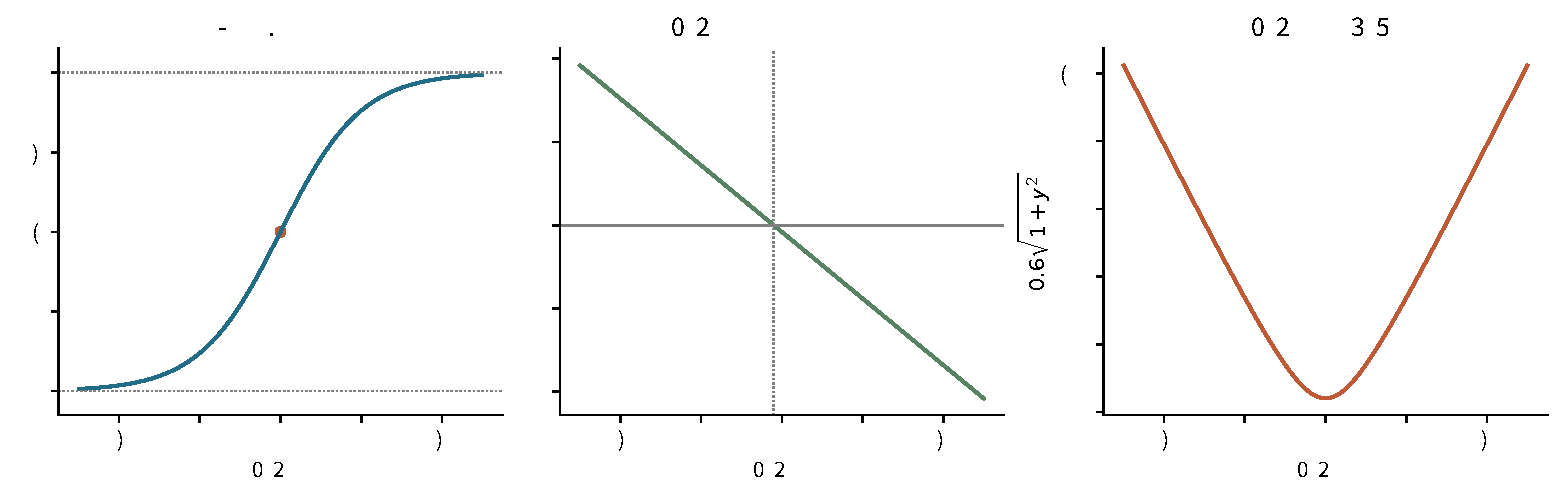
\includegraphics[width=\textwidth]{assets/model_functions.pdf}
\caption{模型函数的含义。左图为有界波动率；中图的正负号决定回复方向；右图是因子的随机扩散幅度。这些是题设函数曲线，不是模拟得到的经验规律。}\label{fig:na-functions}
\end{figure}
图~\ref{fig:na-functions} 将三个容易混淆的函数并列展示：资产的波动率是左图，因子的漂移与扩散分别是中图和右图。

\subsection{相关的布朗运动怎样由独立正态数生成？}
两种随机冲击可以相关，但它们不是同一个冲击。
从相互独立的 $Z_1,Z_2\sim N(0,1)$ 出发，设置
\begin{equation}\label{eq:na-correlated}
 \Delta W^{(1)}=\sqrt h Z_1,\qquad
 \Delta W^{(2)}=\sqrt h\bigl(\rho Z_1+\sqrt{1-\rho^2}Z_2\bigr).
\end{equation}
逐项计算就能验证：
\begin{align}
 \Var(\Delta W^{(2)})&=h\{\rho^2+(1-\rho^2)\}=h,\label{eq:na-driver-var}\\
 \Cov(\Delta W^{(1)},\Delta W^{(2)})&=h\rho,\qquad
 \operatorname{Corr}(\Delta W^{(1)},\Delta W^{(2)})=\rho.\label{eq:na-driver-cov}
\end{align}
原题记号 $d\langle W^{(1)},W^{(2)}\rangle_t=\rho\,dt$ 描述两个驱动的二次协变差：把前面的增量平方和改为同一时段两个增量的乘积和，其极限为 $\rho t$。
在 Itô 运算中，它对应 $dW^{(1)}dW^{(2)}=\rho\,dt$ 的记账规则。
不同时间段仍用新的独立正态对。

$\rho=-0.7$ 的直觉是：驱动价格的冲击偏负时，驱动因子的冲击倾向偏正，于是波动率倾向升高。
这是即时随机冲击的倾向，不是每一条路径的确定规律。
它也不是 $S_T$ 和 $Y_T$ 两个终值的相关系数；后者受整个非线性系统共同影响。
遗漏 $\sqrt{1-\rho^2}$、直接使用 $\rho Z_1+Z_2$，会把第二个增量方差变成 $(1+\rho^2)h$，模拟的是错误模型。

\subsection{“非仿射”具体指什么？}
“仿射”指常数加状态的一次函数。
在仿射扩散模型中，关键通常是漂移和\emph{瞬时协方差矩阵}对状态具有仿射结构，而不只是扩散系数表面上是否有平方根。
因此不能说“出现平方根就一定非仿射”。
本模型的瞬时协方差矩阵如下；在很短的时间 $h$ 内，$(\Delta X,\Delta Y)$ 的条件协方差矩阵近似为它乘以 $h$：
\begin{equation}\label{eq:na-cov-matrix}
 \begin{pmatrix}
  g(y)^2 & \rho\xi g(y)\sqrt{1+y^2}\\
  \rho\xi g(y)\sqrt{1+y^2} & \xi^2(1+y^2)
 \end{pmatrix}.
\end{equation}
其中 $g(y)^2$ 和 $1+y^2$ 不是状态的一次函数，$X$ 的漂移也含 $g(y)^2$，所以不具备该结构。
这个名称主要帮助理解模型类别；写出 EM 并不需要先掌握整个仿射过程理论。

\subsection{对两个状态同步使用左端 EM}
一步开始时已知 $X_n,Y_n$，先计算 $g_n=g(Y_n)$，再使用同一时段的两维增量：
\begin{align}
 X_{n+1}&=X_n+(\mu-g_n^2/2)h+g_n\Delta W_n^{(1)},\label{eq:na-em-x}\\
 Y_{n+1}&=Y_n+\kappa(\theta-Y_n)h+\xi\sqrt{1+Y_n^2}\Delta W_n^{(2)},\label{eq:na-em-y}\\
 S_{n+1}&=e^{X_{n+1}}.\label{eq:na-em-s}
\end{align}
两条式子的系数都使用\emph{旧的} $Y_n$。
若先更新 $Y$，再将 $Y_{n+1}$ 放进 $X$ 的系数，同一步的新噪声就进入了扩散系数，这已改变离散方法。
尤其当两个驱动相关时，这种修改不只是代码顺序的无害变化。

做一次手算：取 $h=0.01$、$X_n=\log100$、$Y_n=0$，这一步 $Z_1=1$、$Z_2=0$。
由式~\eqref{eq:na-correlated} 得 $\Delta W^{(1)}=0.1$、$\Delta W^{(2)}=-0.07$；此时 $g_n=0.3$。
所以
\begin{equation}\label{eq:na-hand-step}
 \Delta X=0.005(0.01)+0.3(0.1)=0.03005,\qquad
 Y_{n+1}=0+2(-0.2)(0.01)+0.6(-0.07)=-0.046.
\end{equation}
价格为 $100e^{0.03005}\approx103.0506$。
新的 $Y=-0.046$ 会影响\emph{下一步}的波动率，不回头改变这一步已经使用的 $0.3$。

在实数运算中，$e^X>0$ 自动成立。在浮点运算中，极端大的 $X$ 可能上溢、极端小的 $X$ 可能下溢到零。
现有程序不仅检查终值，还追踪所有网格步的 $X,Y$ 极值与有限性，确认指数处于可表示的正有限范围。
这比仅看到最终数组没有 NaN 更有说服力。

\subsection{为什么不照搬一维 Milstein？}
将相关驱动写成两个独立布朗运动 $B^{(1)},B^{(2)}$，令 $a(y)=\xi\sqrt{1+y^2}$、$c=\sqrt{1-\rho^2}$，对应扩散向量是
\begin{equation}\label{eq:na-diffusion-columns}
 b_1(x,y)=\binom{g(y)}{\rho a(y)},\qquad b_2(x,y)=\binom{0}{ca(y)}.
\end{equation}
二维随机 Taylor 展开通常还会出现 $\int(B^{(1)}_s-B^{(1)}_{t_n})\,dB_s^{(2)}$ 等交叉迭代积分。
一维时，同一个噪声的迭代积分可化为 $(\Delta W^2-h)/2$；两个不同噪声的交叉信息一般不能仅由两个终点增量恢复。
本模型两种噪声的作用也不满足简化交叉项所需的交换条件。
这里 $Db_j$ 是向量函数 $b_j$ 的一阶偏导组成的矩阵，$(Db_j)b_k$ 衡量沿另一噪声方向移动时 $b_j$ 怎样变化：
\begin{equation}\label{eq:na-noncommute}
 (Db_2)b_1-(Db_1)b_2=\binom{-ca(y)g'(y)}0\ne0.
\end{equation}
初读时只需要记住：把标量修正项分别粘到两个方程上，并不能得到这个系统的强一阶方法。
原题明确要求本模型使用 EM；现有实现遵循这个要求。

\subsection{从理论上为什么预期出现半阶？进阶说明}
函数 $g$ 有界且导数有界，而
$\frac{d}{dy}\sqrt{1+y^2}=y/\sqrt{1+y^2}$ 的绝对值不超过 1。
因此 $(X,Y)$ 系统的漂移和扩散对状态全局 Lipschitz，并满足线性增长界。
标准 EM 理论在这里给出状态的终值均方根误差 $O(\sqrt h)$。

从 $X$ 转回 $S=e^X$ 需要多一步，因为指数函数不是全局 Lipschitz。
利用
\begin{equation}\label{eq:na-exp-error}
 |e^x-e^y|\le(e^x+e^y)|x-y|,
\end{equation}
再应用 Cauchy--Schwarz 不等式：
\begin{equation}\label{eq:na-strong-bound}
 \E|S_T^{(h)}-S_T|
 \le \sqrt{\E[(S_T^{(h)}+S_T)^2]}\,
       \sqrt{\E|X_T^{(h)}-X_T|^2}.
\end{equation}
有界的 $g$ 使第一因子对步长一致有界。例如离散方案满足
$\E[(S_{n+1})^2\mid\mathcal F_{t_n}]=S_n^2e^{2\mu h+g_n^2h}$，
故 $\E[S_N^2]\le S_0^2e^{(2\mu+\sigma_{\max}^2)T}$；连续模型也有同样形式的二阶矩上界。
于是价格终值的 $L^1$ 强误差有 $O(\sqrt h)$ 上界。
这说明半阶有理论依据，但\emph{现有图中直接测量的量}仍然是两个数值解之间的差，不能改称真误差。

\section{没有精确解时，怎样判断数值结果可信？}\label{sec:reference}
\subsection{三个参考网格也必须共享同一套噪声}
现有非仿射实验有 $100000$ 条路径。
粗网格步数为 $8,16,32,64,128,256$，参考网格步数为 $2048,4096,8192$。
程序先在 $8192$ 步生成两维相关增量，再通过相邻求和生成\emph{所有}其他网格。
三个参考仍是 EM，只是步长更小；较细并不意味着数学上精确。

设未知真解终值为 $S_T^\star$，粗解为 $S_T^{(h)}$，参考为 $S_T^{(r)}$。
三角不等式及反三角不等式给出
\begin{equation}\label{eq:ref-triangle}
 \left|\E|S_T^{(h)}-S_T^\star|-\E|S_T^{(h)}-S_T^{(r)}|\right|
 \le\E|S_T^{(r)}-S_T^\star|.
\end{equation}
右侧才是参考真误差，却是未知的。
将 $r$ 加密到 $r/2$，能观察的是 $\E|S_T^{(r)}-S_T^{(r/2)}|$。
它是参考敏感度的证据，不是式~\eqref{eq:ref-triangle} 右侧的已知上界。
如果两个参考共享相似的离散误差，它们可以非常接近而仍共同偏离真解。

\subsection{现有的 10\% 筛查应怎样理解？}
最后两层参考之间的平均绝对差为 $0.04015705$。
现有报告将它除以各粗网格相对最细参考的强差，作为一个实践性比例：
\begin{equation}\label{eq:ref-screen}
 R_h=\frac{\widehat\E|S_T^{(1/4096)}-S_T^{(1/8192)}|}
 {\widehat\E|S_T^{(h)}-S_T^{(1/8192)}|}.
\end{equation}
在预先指定的主拟合窗口 $N=8,16,32,64$，该比值约为 $3.20\%,4.46\%,6.29\%,8.89\%$，都低于 10\%。
到了 $N=128,256$，则约为 $12.61\%,17.99\%$，说明更细的粗网格相对更加受参考分辨率影响。

10\% 不是随机分析定理给出的万能阈值，而是原实验使用的敏感度标准。
正确结论是“主窗口对最后一次参考加密的变化相对不太敏感”，不是“参考真误差已被严格证明低于粗误差的 10\%”。
两个连续加密差从 $0.05679005$ 降到 $0.04015705$，比例约为 $0.7071$，与半阶缩放相容。
这仍然是数值证据；没有额外渐近假设或误差界，不能将其中一个差直接变成严格误差证书。

\subsection{为什么本模型不能再只检查价格均值？}
对 $S=e^X$ 应用 Itô 公式：
\begin{equation}\label{eq:ref-price-sde}
 dS_t=S_t\left[(\mu-g(Y_t)^2/2)dt+g(Y_t)dW_t^{(1)}\right]
       +\frac12S_tg(Y_t)^2dt
 =\mu S_tdt+g(Y_t)S_t\,dW_t^{(1)}.
\end{equation}
有界波动率提供足够的可积性，使随机积分均值为零；因此 $\E S_T=S_0e^{\mu T}$。
严格地说，可以先由有界 $g$ 得到有限二阶矩，再对积分方程取期望，解线性积分方程。

更特别的是，log-EM 也保留这个均值。
在第 $n$ 步开始时，$S_n$ 和 $g_n=g(Y_n)$ 都已知。
下一步 $\Delta W_n^{(1)}$ 与过去信息独立，条件下服从 $N(0,h)$，所以
\begin{equation}\label{eq:ref-discrete-mean}
\begin{aligned}
 \E[S_{n+1}\mid\mathcal F_{t_n}]
 &=S_ne^{(\mu-g_n^2/2)h}\E[e^{g_n\Delta W_n^{(1)}}\mid\mathcal F_{t_n}]\\
 &=S_ne^{(\mu-g_n^2/2)h}e^{g_n^2h/2}=e^{\mu h}S_n.
\end{aligned}
\end{equation}
反复取期望，所有步长都得到 $\E S_N=S_0e^{\mu T}$。
两个布朗驱动之间的相关性不妨碍这个计算，因为当前 $Y_n$ 只依赖过去，而不是下一步的增量。
这也解释了为什么同步左端更新如此关键。

所以，均值偏离目标可能提示抽样波动或实现问题，但均值符合目标不能识别本方法的离散偏差。
单条路径仍可能不准，其他分布特征也可能不准。

\subsection{用看涨收益观察非线性的分布信息}
题目选择
\begin{equation}\label{eq:ref-payoff}
 \varphi(s)=(s-100)^+=\begin{cases}0,&s\le100,\\s-100,&s>100.\end{cases}
\end{equation}
价格低于 100 时收益为零，高于 100 时只取超过部分。
例如终值 $90,100,120$ 分别对应收益 $0,0,20$。
这个函数会区分价格分布在执行价两侧的形状，不再只依赖一阶矩。
但它在 100 处不可微，不能未经论证直接套用要求测试函数光滑的弱收敛结论。

统计时对每条共同路径计算 $D_i=(S_{T,i}^{(h)}-100)^+-(S_{T,i}^{(r)}-100)^+$，再求有符号均值和置信区间。
函数 $\varphi$ 是 1-Lipschitz 的，即 $|\varphi(u)-\varphi(v)|\le|u-v|$，因此
\begin{equation}\label{eq:ref-payoff-bound}
 |\E\varphi(S_T^{(r)})-\E\varphi(S_T^\star)|
 \le\E|S_T^{(r)}-S_T^\star|,
\end{equation}
但右侧仍然未知，采样区间依旧没有覆盖参考偏差的自动保证。

现有最细参考的收益均值约为 $14.5380$，其抽样区间约为 $[14.4052,14.6709]$。
这个量是给定模型漂移下的\emph{未贴现期望收益}。
若要称为某一风险中性模型下的期权价格，还需要说明定价测度与无风险贴现率等条件；本题没有完成这些额外设定。
这里研究的是数值积分和统计估计，不应额外赋予定价含义。


\section{进阶：逐项理解 GBM 程序中的五个控制变量}\label{sec:controls}
\subsection{先掌握一个控制变量的原理}
设我们想估计 $b=\E D$，又找到了一个期望已知为零的随机变量 $C$。
对任意事先固定的常数 $\beta$，
\begin{equation}\label{eq:cv-unbiased}
 \E[D-\beta C]=\E D-\beta\E C=b.
\end{equation}
均值不变，方差却能改变：
\begin{equation}\label{eq:cv-variance}
 \Var(D-\beta C)=\Var D-2\beta\Cov(D,C)+\beta^2\Var C.
\end{equation}
若 $\Var C>0$，对 $\beta$ 求导，最优值为 $\beta_\star=\Cov(D,C)/\Var C$。
当 $C$ 与 $D$ 高度相关时，减去 $\beta C$ 就像消除误差中可预测的随机波动，只留下较小的剩余噪声。
例如若 $D=b+3C+\varepsilon$，且 $\E\varepsilon=0$、$\varepsilon$ 独立于 $C$，选择 $\beta=3$ 后得到 $b+\varepsilon$。
这个例子也说明我们没有把未知常数 $b$ 预先塞入估计。

多个控制组成列向量 $C$，相应最优系数满足
\begin{equation}\label{eq:cv-vector}
 \Cov(C,C)\beta=\Cov(C,D),\qquad D_{\mathrm{cv}}=D-\beta^\top C.
\end{equation}
程序用独立的 $20000$ 条预实验路径估计协方差、解这个线性系统，再把系数固定，用于 $160000$ 条正式路径。
不同网格、不同方法各有一套系数。
条件于预实验得到的 $\widehat\beta$，正式样本与之独立，故
\begin{equation}\label{eq:cv-pilot}
 \E[D-\widehat\beta^\top C\mid\widehat\beta]=\E D.
\end{equation}
若直接在同一批最终数据上拟合并评估，一般不能不加论证地沿用这个独立性证明。
独立预实验有清楚的理论好处，代价是增加一次较小的计算。

\subsection{指数加权其实只是给正态密度配方}
在一个固定网格上，记
\begin{equation}\label{eq:cv-defs}
\begin{aligned}
 W&=\sum_{n=0}^{N-1}\Delta W_n,\qquad
 L=e^{\sigma W-\sigma^2T/2}=\frac{S_T^{\mathrm{exact}}}{\E S_T},\\
 Q&=\sum_{n=0}^{N-1}\bigl((\Delta W_n)^2-h\bigr),\qquad
 R=\sum_{n=0}^{N-1}\bigl((\Delta W_n)^3-3h\Delta W_n\bigr).
\end{aligned}
\end{equation}
已经知道 $\E L=1$。$Q$ 是二次变差与 $T$ 的差，$R$ 是去掉主要线性部分的三次增量和。
EM 和 Milstein 误差的展开自然包含这些二次、三次项，所以它们适合帮助预测误差波动。

为了计算 $LQ$ 等量的期望，对单个 $u=\Delta W_n\sim N(0,h)$ 配方：
\begin{equation}\label{eq:cv-tilt-density}
 e^{\sigma u-\sigma^2h/2}\frac1{\sqrt{2\pi h}}e^{-u^2/(2h)}
 =\frac1{\sqrt{2\pi h}}e^{-(u-\sigma h)^2/(2h)}.
\end{equation}
右边恰好是 $N(\sigma h,h)$ 的密度。
因为 $T=Nh$，把所有独立增量的密度相乘，就能把 $L$ 分配到每一个增量上。
于是对满足 $\E[L|F|]<\infty$ 的函数 $F$ 有（后面使用的多项式都满足这一条件）
\begin{equation}\label{eq:cv-tilt-identity}
 \E[L F(\Delta W_0,\ldots,\Delta W_{N-1})]
 =\widetilde\E[F(U_0,\ldots,U_{N-1})],
\end{equation}
其中右侧只是记号：$U_n$ 相互独立、服从 $N(\sigma h,h)$。
这里用到的是普通概率密度配方，不要求先学习一般的测度变换定理；实际仿真也没有改成从这个偏移正态分布抽样。

\subsection{把所需的期望逐个算出来}
令 $m=\sigma h$，则在加权后的计算中 $U=m+\sqrt h Z$。
利用标准正态的 $\E Z=\E Z^3=0$、$\E Z^2=1$、$\E Z^4=3$，得到
\begin{align}
 \widetilde\E U&=m,\quad \widetilde\E U^2=h+m^2,
 \quad\widetilde\E U^3=m^3+3mh,\label{eq:cv-gaussian-low}\\
 \widetilde\E U^4&=m^4+6m^2h+3h^2,\qquad
 \widetilde\Var(U^2)=2h^2+4m^2h.\label{eq:cv-gaussian-fourth}
\end{align}
对 $N=T/h$ 个独立增量求和，就有
\begin{align}
 \widetilde\E W&=\sigma T,\label{eq:cv-ew}\\
 \widetilde\E Q&=Nm^2=\sigma^2Th,\label{eq:cv-eq}\\
 \widetilde\E R&=Nm^3=\sigma^3Th^2,\label{eq:cv-er}\\
 \widetilde\Var Q&=N(2h^2+4\sigma^2h^3)=2Th+4\sigma^2Th^2,\label{eq:cv-varq}\\
 \widetilde\E Q^2&=\widetilde\Var Q+(\widetilde\E Q)^2
 =2Th+4\sigma^2Th^2+\sigma^4T^2h^2.\label{eq:cv-eq2}
\end{align}
关键区别是：原分布下 $\E Q=0$，但 $\E[LQ]$ 不为零，因为 $L$ 与 $Q$ 相关。
因此不能把 $LQ$ 直接当作零均值控制，必须减去\emph{加权分布下}的中心值。

\subsection{与程序一一对应的控制向量}
现有 \texttt{simulate\_batch} 函数构造以下五列：
\begin{align}
 C_1&=L-1,\label{eq:cv-c1}\\
 C_2&=\frac{L(W-\sigma T)}{\sqrt T},\label{eq:cv-c2}\\
 C_3&=\frac{L(Q-\sigma^2Th)}{\sqrt{2Th}},\label{eq:cv-c3}\\
 C_4&=\frac{L(R-\sigma^3Th^2)}{\sqrt{6Th^2}},\label{eq:cv-c4}\\
 C_5&=\frac{L\{Q^2-(2Th+4\sigma^2Th^2+\sigma^4T^2h^2)\}}{\sqrt8\,Th}.\label{eq:cv-c5}
\end{align}
由式~\eqref{eq:cv-tilt-identity} 和刚才逐项求得的期望，每一列都严格满足 $\E C_j=0$。
分母用于平衡各列的数值尺度，\emph{不表示加权后的每一列方差恰好等于 1}。
把某列乘以一个非零常数，再相应调整回归系数，不改变控制变量方法的基本原理。

程序用正式样本的 $D_{\mathrm{cv}}$ 计算均值、样本标准差和置信区间，使用的是实际残差的波动。
解析偏差只放在另一列作核对目标，并没有代替正式蒙特卡洛估计。
粗糙的 $\widehat\beta$ 可能使方差减少不充分，却不会在独立性条件下改变估计期望。

\subsection{为什么这里降噪会特别明显？}
GBM 有极强的解析结构：误差和这些低阶增量组合高度相关。
最细网格的 EM 原始配对标准误差约为 $5.464\times10^{-4}$，控制后约为 $8.415\times10^{-8}$。
方差比约为 $4.216\times10^7$；它是标准误差比的平方，不能直接当作标准误差减少倍数。
这样的效果是本模型、本控制设计和当前网格共同造成的，不能保证任意模型都有同样收益。



\section{把公式落实到现有 Python 项目}
\label{code:chapter}

这一节按实际计算顺序阅读现有代码。先理解一个数组代表什么，再看如何更新状态，最后看误差怎样汇总成报告。这里的短代码取自原程序或本讲义附带的教学脚本；为便于阅读而省略上下文的片段不应单独当作完整程序运行。原项目解决大规模实验与报告生成，新增的 \texttt{teaching\_demo.py} 则保留学习所需的核心计算，只依赖 NumPy，默认打印结果，不写文件。

\subsection{文件之间怎样配合}

\begin{center}
\small
\begin{tabularx}{\textwidth}{@{}lY@{}}
\toprule
文件 & 职责与阅读重点\\
\midrule
\texttt{gbm.py} & 生成共同布朗增量；计算精确 GBM、价格 EM、Milstein；独立预试验拟合控制变量；保存收敛统计、终值样本和图。\\
\texttt{nonaffine.py} & 生成相关布朗增量；对 $(X,Y)$ 做 log-EM；比较粗网格与三层参考网格；记录状态与参考敏感性。\\
\texttt{verify.py} & 用确定性输入和另一种写法核对算法，再由保存的终值数组重新算误差，检查统计是否一致。\\
\texttt{build\_report\_data.py} & 从已有 JSON/CSV 生成报告使用的数值宏、八张表和四幅图，并更新 \texttt{numerical\_summary.txt}。\\
\texttt{run\_all.py} & 依次运行上面四个脚本；某一步失败就停止；它本身不编译 \LaTeX。\\
\texttt{README.md} & 记录依赖、实验规模、命令、误差定义和解释边界。\\
\bottomrule
\end{tabularx}
\end{center}

\texttt{results/} 保存计算结果，\texttt{figures/} 保存图，原报告的 \texttt{.tex} 把这些结果排版。因而“重画已有结果”“重新模拟所有路径”“重新编译 PDF”是三个不同操作。原项目的这几个生成脚本使用固定输出文件名；学习时先运行新增教学脚本，可以保留现有实验结果。

\subsection{NumPy 数组：先问每一个轴代表什么}

NumPy 的 \texttt{array} 是规则排列的数。\texttt{shape} 给出每个轴上的长度，轴编号从 0 开始。设本批有 $B$ 条独立路径，最细网格有 $N_f$ 步。GBM 使用“路径在前”的数组：
\begin{lstlisting}[language=Python]
fine = rng.normal(0, math.sqrt(T / nfine), (size, nfine))
w = fine.sum(axis=1)
\end{lstlisting}
这里 \texttt{size} 就是 $B$。\texttt{fine.shape == (B, Nf)}，\texttt{fine[j,k]} 是第 $j$ 条路径、第 $k$ 个小时间段的布朗增量。每一行是一条路径。正态生成器的第二个参数是\emph{标准差}，所以传入 $\sqrt{T/N_f}$，不是方差 $T/N_f$。沿 \texttt{axis=1} 求和，就是把每一行的所有时间增量相加，得到 $W_T$；结果 \texttt{w.shape == (B,)}。

若粗网格有 $N$ 步，且 $r=N_f/N$ 是整数，原代码写作
\begin{lstlisting}[language=Python]
dw = fine.reshape(size, int(n), nfine // int(n)).sum(axis=2)
\end{lstlisting}
\texttt{reshape} 不重新抽随机数，它把原有顺序整理为 $(B,N,r)$。最后一个轴含有同一粗区间内连续的 $r$ 个细增量；沿该轴求和，输出 $(B,N)$。例如单条路径八个细增量为
\[
(a_1,a_2,a_3,a_4,a_5,a_6,a_7,a_8),
\]
取 $N=2$ 时，先分为 $(a_1,\ldots,a_4)$ 与 $(a_5,\ldots,a_8)$，再变为 $(a_1+\cdots+a_4,a_5+\cdots+a_8)$。这是“粗细路径共用同一布朗运动”的代码实现。若另抽一套粗增量，即使分布正确，逐路径的差也不再衡量同一随机驱动下的离散误差。

非仿射程序则使用“时间在前”的数组。两种布局都正确，但求和轴不同：
\begin{center}
\small
\begin{tabularx}{\textwidth}{@{}lYY@{}}
\toprule
操作 & GBM & 非仿射模型\\
\midrule
最细增量形状 & $(B,N_f)$ & $(N_f,B,2)$\\
一个元素 & 第 $j$ 条路径、第 $k$ 步 & 第 $k$ 步、第 $j$ 条路径、第 $q$ 个噪声\\
粗化前重新分组 & $(B,N,r)$ & $(N,r,B,2)$\\
应求和的轴 & \texttt{axis=2} & \texttt{axis=1}\\
粗化后形状 & $(B,N)$ & $(N,B,2)$\\
\bottomrule
\end{tabularx}
\end{center}
不要只背 \texttt{axis=1} 或 \texttt{axis=2}；应先写出形状，再指认“要合并的细时间轴”。类似地，\texttt{sum(axis=0)} 在 $(B,2)$ 上是跨路径汇总，结果中保留两种方法。

\subsection{GBM：从递推式到 \texttt{prod}}

因为 GBM 的系数都正比于价格，价格 EM 和 Milstein 都能写为“旧价格乘一个因子”。原 \texttt{simulate\_batch} 的核心是：
\begin{lstlisting}[language=Python]
exact = S0 * np.exp((MU - 0.5 * SIGMA**2) * T + SIGMA * w)
dw2 = dw * dw
base = 1 + MU * h + SIGMA * dw
em = S0 * np.prod(base, axis=1)
mil = S0 * np.prod(
    base + 0.5 * SIGMA**2 * (dw2 - h), axis=1)
endpoints = np.column_stack((em, mil))
\end{lstlisting}
\texttt{dw*dw} 是每个位置分别平方，\texttt{**2} 也是平方；它们不是矩阵乘法。\texttt{base} 的形状为 $(B,N)$，沿时间轴调用 \texttt{prod}，把每条路径的 $N$ 个乘子相乘，一次得到所有终值。数学上就是
\[
S_N=S_0F_0F_1\cdots F_{N-1}
\]
的简写，没有改变递推格式。若要画整条路径，需要 \texttt{cumprod} 保存逐步累积乘积；终值误差实验只需 \texttt{prod}。精确路径图类似地用 \texttt{cumsum} 得到各时刻的布朗运动。

\texttt{column\_stack} 把两个长度为 $B$ 的数组并成两列，所以 \texttt{endpoints.shape == (B,2)}，第 0 列为 EM，第 1 列为 Milstein。精确终值 \texttt{exact} 的形状却是 $(B,)$。作差时要写
\begin{lstlisting}[language=Python]
error = endpoints - exact[:, None]
\end{lstlisting}
\texttt{:} 表示取全部路径，\texttt{None} 插入一个新轴，令形状从 $(B,)$ 变为 $(B,1)$。NumPy 的广播机制把这一列用于两列数值解，得到 $(B,2)$ 的配对误差。它没有给每种方法重新生成一条精确路径。例如两条路径有
\[
\texttt{endpoints}=\begin{pmatrix}99&100\\110&112\end{pmatrix},
\quad \texttt{exact[:,None]}=\begin{pmatrix}101\\111\end{pmatrix},
\quad \texttt{error}=\begin{pmatrix}-2&-1\\-1&1\end{pmatrix}.
\]
这里的减法在“相同路径”内完成，这是配对估计。

\texttt{simulate\_batch} 中的 \texttt{yield} 使函数成为生成器。调用者用 \texttt{for} 逐层取出四项：步数 $N$、精确终值、两列数值终值、控制变量。程序不会一次保存每个网格的所有中间状态；所有网格共享本批已经生成的 \texttt{fine}。

\subsection{强误差、弱偏差、控制变量各占哪一列}

原程序没有把全部误差样本永久保存在内存，而是对三个指标累积总和与平方和：
\begin{lstlisting}[language=Python]
corrected = error - controls @ betas[k]
metrics = np.stack((np.abs(error), error, corrected), axis=2)
sums[k] += metrics.sum(axis=0)
squares[k] += (metrics * metrics).sum(axis=0)
\end{lstlisting}
此处 \texttt{metrics.shape == (B,2,3)}：第一个轴是路径，第二个轴是方法，第三个轴依次是绝对终值误差、带符号配对差、控制变量修正后的带符号差。跨路径求和后形状为 $(2,3)$。外层 \texttt{sums.shape == (L,2,3)}，其中 $L$ 是网格层数，\texttt{k} 指当前网格。

三列对应的总体目标依次是 $\E|S_T^h-S_T|$、$\E[S_T^h-S_T]$、以及同一个弱偏差。后两列目标相同，估计噪声不同。不能把 \texttt{np.abs(error)} 当成弱误差，也不能先将弱样本逐个取绝对值再平均。

在某一网格上，\texttt{controls.shape == (B,5)}，\texttt{betas[k].shape == (5,2)}。符号 \texttt{@} 表示矩阵乘法，故乘积是 $(B,2)$，为每条路径、每种方法分别计算五个控制变量的加权和。控制变量的严格零均值及方差缩减原理在理论部分已说明；对应代码的关键是：\emph{系数只在独立预试验中拟合，然后在正式样本中固定使用。}

\texttt{fit\_controls} 分批记录 $X$ 与 $Y$ 的总和、$X^TX$ 和 $X^TY$。$X$ 的五列是控制变量，$Y$ 的两列是 EM/Milstein 配对误差。总预试验样本数记为 $M_0$，最终进行中心化最小二乘：
\begin{lstlisting}[language=Python]
covx = sxx[k] - np.outer(sx[k], sx[k]) / count
covxy = sxy[k] - np.outer(sx[k], sy[k]) / count
betas[k] = np.linalg.solve(covx, covxy)
\end{lstlisting}
\texttt{outer} 是外积；例如两个长度分别为 5 和 2 的向量，外积为 $5\times2$ 矩阵。这里 \texttt{covx} 与 \texttt{covxy} 是尚未除以 $M_0-1$ 的中心化交叉乘积；同一个分母会在最小二乘方程两边抵消。\texttt{solve(A,B)} 求解 $AZ=B$，不必显式计算矩阵逆。预试验点数过少会使拟合不稳定，不能随意用几条路径代替原来的 20,000 条预试验路径。

原代码分别使用 \texttt{default\_rng(SEED+1)} 和 \texttt{default\_rng(SEED)} 建立预试验与正式实验的随机流。拟合阶段的中心化用于估计协方差；正式校正时使用理论已知为零均值的控制变量本身，不是用正式样本估计一个均值后再从每个控制变量中扣除。

\subsection{批量累计：平均数和标准误怎样得到}

如果 $V_1,\ldots,V_M$ 是不同路径上的某个指标，只需保存
\[
M,\qquad A=\sum_{j=1}^M V_j,\qquad B_2=\sum_{j=1}^M V_j^2,
\]
就能计算
\begin{equation}
\overline V=\frac{A}{M},\qquad
s^2=\frac{B_2-A^2/M}{M-1},\qquad
\operatorname{SE}(\overline V)=\frac{s}{\sqrt M}.
\label{code:streaming}
\end{equation}
\texttt{gbm.py} 的 \texttt{mean\_se(total,squares,count)} 把这三个公式一次应用到所有网格、方法、指标。\texttt{np.maximum(...,0)} 避免理论上非负的方差因浮点舍入产生很小的负数；它不能修复错误的数据。

非仿射程序把同一逻辑封装进 \texttt{Moments} 对象，其接口是：
\begin{lstlisting}[language=Python]
strong[n, r].add(np.abs(terminal[n] - terminal[r]))
weak[n, r].add(payoff[n] - payoff[r])
result = strong[n, r].summary()
\end{lstlisting}
\texttt{add(values)} 接收一批独立路径的观测值，更新样本数、总和与平方和；\texttt{summary()} 返回均值、标准误、95\% 区间上下端点等字段。上式字典的键 \texttt{(n,r)} 表示“粗网格 $n$ 步，对照参考网格 $r$ 步”。元组键不是乘法。

这样分批的统计结果与把所有样本放在一起平均等价，只有浮点加法顺序带来的微小差别。分批还能限制布朗增量数组的内存占用。不过原项目为绘图和事后检查，另外保留了部分或全部终值样本；它并不是完全不存样本。若数据均值极大、方差极小，式 \eqref{code:streaming} 的两大数相减会损失精度，可改用 Welford 算法；现有程序采用的是总和与平方和形式。

跨网格数据相关，因为它们共用布朗路径；同一网格上不同路径仍是 Monte Carlo 平均所用的独立观测。因此逐点标准误有明确意义，但各层 95\% 区间不是“所有层同时覆盖真值的 95\% 区间”。

\subsection{非仿射模型：相关噪声和同时更新}

\texttt{nonaffine.py} 首先生成两个独立标准正态数组，然后在线性组合中加入相关性：
\begin{lstlisting}[language=Python]
dw = rng.standard_normal((finest, m, 2))
dw[:, :, 1] = (
    PARAMETERS["rho"] * dw[:, :, 0]
    + math.sqrt(1 - PARAMETERS["rho"]**2) * dw[:, :, 1])
dw *= math.sqrt(hfinest)
\end{lstlisting}
赋值右侧计算时，\texttt{dw[:,:,1]} 还是原先独立的第二个正态噪声。令 $Z_1,Z_2$ 独立标准正态，则最终的两个增量为
\[
\Delta W_1=\sqrt h Z_1,\qquad
\Delta W_2=\sqrt h\bigl(\rho Z_1+\sqrt{1-\rho^2}Z_2\bigr).
\]
直接用概率论可核对：两者方差均为 $h$，协方差为 $\rho h$，相关系数为 $\rho$。这里的第三个轴长度为 2，记录两种噪声；“路径条数很多”不等于“每条路径有很多独立噪声分量”。

\texttt{em\_terminal} 将最细网格增量按时间分组：
\begin{lstlisting}[language=Python]
finest, n_paths, _ = dw.shape
ratio = finest // n_steps
increments = dw if ratio == 1 else dw.reshape(
    n_steps, ratio, n_paths, 2).sum(axis=1)
\end{lstlisting}
如果本层已经是最细网格，直接复用原数组；否则将相邻细增量相加。原实验的所有步数都整除 8192；教学脚本另外显式检查整除关系，避免误用不相容的网格。

在计算内核里，\texttt{x} 保存 $X=\log S$，\texttt{y} 保存 $Y$。对每个时刻、每条路径，原程序用旧状态计算两个新状态：
\begin{lstlisting}[language=Python]
old_y = y[j]
g = g_min + (g_max - g_min) * sigmoid
x[j] += (mu - 0.5*g*g)*h + g*increments[step, j, 0]
y[j] += (kappa*(theta-old_y)*h
         + xi*math.sqrt(1.0+old_y*old_y)*increments[step, j, 1])
\end{lstlisting}
这里 \texttt{sigmoid} 也是在 \texttt{old\_y} 上计算的。\texttt{+=} 表示将右侧增量加到左侧旧值。代码先写 $X$ 更新、再写 $Y$ 更新，并不意味着第二个公式使用了新 $Y$；两个公式的系数都在 $Y_n$ 上取值。这正是“同时更新”的含义。若先改写 $Y$、再用新 $Y$ 计算波动率，就已经换成了另一种离散方法。

教学脚本对全部路径一次进行向量运算，写 \texttt{old\_y = y.copy()} 后再更新。这里需要 \texttt{copy()} 的原因是：\texttt{old\_y = y} 只让两个变量名指向同一个数组；后续原地修改 \texttt{y} 会同时改变它。原 Numba 内核里的 \texttt{old\_y = y[j]} 是标量读取，不存在这个数组别名问题。

逻辑函数 $\ell(y)=1/(1+e^{-y})$ 的稳定计算也值得读懂：
\begin{lstlisting}[language=Python]
if old_y >= 0:
    sigmoid = 1.0 / (1.0 + math.exp(-old_y))
else:
    exp_y = math.exp(old_y)
    sigmoid = exp_y / (1.0 + exp_y)
\end{lstlisting}
$y\geq0$ 时 $-y\leq0$，$y<0$ 时直接算 $e^y$，所以两分支都不会计算极大的正指数。两式数学上相等，但这样避免 $y$ 很负时 $e^{-y}$ 溢出。教学脚本用布尔掩码实现同样的两分支；不直接用可能同时计算两边的 \texttt{np.where}。最终才用 \texttt{np.exp(x)} 还原价格，并检查其有限性与正性。理论上的 $e^x>0$ 不会自动阻止计算机上的上溢或下溢，因此原项目也记录中间 $X,Y$ 的范围和状态诊断。

\subsection{为什么原非仿射代码使用 Numba}

原非仿射实验包含 100,000 条路径，以及 $N=8,16,32,64,128,256,2048,4096,8192$ 共九层网格。总路径步更新数为
\[
100000\,(8+16+32+64+128+256+2048+4096+8192)
=1\,484\,000\,000.
\]
纯 Python 的双重逐项循环开销较大。\texttt{@njit(cache=False)} 让 Numba 在首次调用时把内核编译为较快的机器代码；公式没有因编译而改变。\texttt{run} 先用一个很小的零增量输入预热编译，并单独记录编译耗时，再开始统计主实验时间。因此不能只比较两个脚本日志里的秒数，就宣称某种数学方法更快：样本数、网格、绘图和预试验范围本来不同。

教学脚本去掉 Numba，时间步仍循环，但在每一步使用 NumPy 同时更新整批路径。它的较小网格足以学习算法，也能在本机当前 Python/NumPy 环境中直接运行。它不会冒充原来十万路径、最细 8192 步的大规模实验。

\subsection{结果文件、日志与报告数字怎样连接}

\texttt{CSV} 是带列名的表格，例如 \texttt{gbm\_convergence.csv} 每行对应一种方法和一个网格，并分别保存强误差、原始弱偏差、控制变量弱偏差及其标准误。\texttt{JSON} 适合嵌套结构：参数、随机种子、软件版本、拟合窗口、诊断和结果可以放进同一份摘要。\texttt{NPZ} 是 NumPy 的压缩数组容器，保存真实终值样本，便于事后从样本重新计算统计。

例如原非仿射结果存为 \texttt{nonaffine\_terminals.npz}，其中键 \texttt{S\_64} 表示 64 步网格的全部终值，\texttt{S\_8192} 表示最细参考的全部终值。下面是一段\emph{只读}练习，须在项目根目录运行：
\begin{lstlisting}[language=Python]
from pathlib import Path
import numpy as np

with np.load(Path("results") / "nonaffine_terminals.npz") as data:
    coarse = data["S_64"]
    reference = data["S_8192"]
    strong = np.mean(np.abs(coarse - reference))
    difference = (np.maximum(coarse - 100.0, 0.0)
                  - np.maximum(reference - 100.0, 0.0))
    weak = difference.mean()
    se = difference.std(ddof=1) / np.sqrt(difference.size)
print(strong, weak, se)
\end{lstlisting}
\texttt{maximum(s-100,0)} 是逐元素计算看涨收益。\texttt{ddof=1} 表示样本方差用分母 $M-1$。标准误必须从\emph{配对差} \texttt{difference} 计算，不能忽略粗细样本的协方差。

\texttt{verify.py} 就包括这种保存结果的交叉检查，还用预先指定的正弦、余弦小数组比较“向量化写法”和“逐条递推写法”。这些小数组不是布朗运动样本；它们的用途是检验代数实现，不是检验随机模型的分布。它还检查常波动率情况下 log-EM 是否退化为精确 GBM。通过后写入 \texttt{results/verification.json}。该脚本会导入 \texttt{nonaffine.py}，因此也需要 Numba；它不会重新模拟全部路径，但不是完全不写文件的检查。

\texttt{build\_report\_data.py} 不再抽样，而是读 JSON/CSV，生成 \texttt{report\_values.tex} 与各表格的 \texttt{.tex}，并更新报告图。这让报告中“EM 强阶”等数字直接来自保存结果。用 \texttt{np.polyfit} 对 $\log h$ 与 $\log e$ 作一次直线拟合，返回斜率与截距；斜率对应经验幂指数。程序对非仿射弱差先检查选定窗口中的区间是否排除零；若有区间含零，\texttt{rate\_fit} 返回 \texttt{slope=None}。即使均排除零，原程序仍将有限参考下的斜率标为描述性结果。

GBM 的 \texttt{log} 函数一边打印、一边把内容加入列表，最后写入 \texttt{gbm\_run.log}。非仿射程序打印进度和摘要，并把时间、种子与环境写进 JSON；\texttt{run\_all.py} 本身没有把所有终端输出自动收集成总日志。需要记录个人演示输出时，可明确重定向到讲义目录中的新文件。

\subsection{从小练习开始，再决定是否完整复现实验}

本讲义新增 \texttt{tutorial\_zh/teaching\_demo.py}。在项目根目录打开终端，依次运行：
\begin{lstlisting}[language=bash]
python3 tutorial_zh/teaching_demo.py --self-check
python3 tutorial_zh/teaching_demo.py
python3 tutorial_zh/teaching_demo.py --paths 8000 --seed 2026090804
\end{lstlisting}
第一条只执行确定性检查，包括 GBM 递推与精确公式、粗化后总增量一致、非仿射旧状态同时更新、常波动率退化、极端输入下逻辑函数稳定性，以及分批统计的标准误。第二条默认使用 2000 条路径、批大小 256；GBM 的层数为 $8,16,\ldots,512$，非仿射粗网格为 $16,32,64,128$，参考网格为 $256,512,1024$。第三条增加路径数，适合观察区间通常如何缩窄。脚本没有控制变量，也不自动拟合或认证收敛阶。

本次在本机 Python 3.9.6、NumPy 2.0.2 上，确定性检查通过，默认演示运行通过。例如 GBM 的 $N=512$ 时，EM 强误差约为 $0.236916$，Milstein 约为 $0.003028$；EM 的原始弱差约为 $-0.001314$，其 95\% 区间约为 $[-0.014883,0.012255]$，而解析均值偏差约为 $-0.000257$。这个小练习同时展示了“强误差明显可见”和“弱偏差可能被抽样噪声淹没”。这些是教学脚本自己的结果，不替换原报告的统计数字。

非仿射演示的参考只到 1024 步，默认样本中 $512\to1024$ 的平均绝对终值差约为 $0.116254$。与某个粗网格差相比，它可能并不小；这正好提醒我们检查参考误差，不能把最细曲线直接命名为精确解。更换种子后个别区间或误差大小会变化，不应要求每次结果都整齐地单调下降。

原项目完整运行使用 README 中记录的依赖环境。其 \texttt{requirements.txt} 固定 NumPy、Matplotlib 和 Numba 版本；已有实验元数据来自另一套环境，因此本机能运行 NumPy 教学版，并不表示已复现原环境。准备好兼容依赖、并在项目的副本中操作时，完整实验命令为：
\begin{lstlisting}[language=bash]
python3 run_all.py
\end{lstlisting}
或者分别执行：
\begin{lstlisting}[language=bash]
python3 gbm.py --paths 160000 --pilot-paths 20000 --batch-size 2000
python3 nonaffine.py --paths 100000 --batch-size 512 --seed 2026090804
python3 verify.py
python3 build_report_data.py
\end{lstlisting}
原 GBM 的种子写在常量 \texttt{SEED} 中，没有 \texttt{--seed} 命令行选项。非仿射与教学脚本有该选项。原报告源是英文，可按其 README 用 \texttt{pdflatex} 编译；本中文讲义采用支持中文的引擎，编译方法见随讲义生成的说明。

最后要区分“同分布复现实验”和“尽量得到同一串输出数字”。固定种子决定伪随机流，但还应保留生成器类型、软件版本、路径数、网格、批大小及抽样调用顺序。非仿射数组是 $(N_f,B,2)$；改变 $B$ 后，同一串随机数会分配到不同的路径和时间位置，所以即使种子相同，逐路径终值仍会改变。GBM 与非仿射在原项目中使用相同种子，也不意味着二者共享可逐路径比较的噪声；它们是两个不同实验。教学脚本有意分别使用传入的种子及其加一值，并将它们打印出来。

建议实际练习时先读清一批的数组形状，再手算一条两步路径，接着核对默认输出中的强误差与带符号弱差，最后查看保存终值能否还原原报告统计。这样每一层代码都有可解释、可核对的数学对象。


\section{逐项读懂现有图表与实际实验结果}\label{sec:results}
\subsection{先确认实验规模，再看小数点}
GBM 的正式路径数为 $160000$，独立控制变量预实验为 $20000$ 条；最细网格为 $1024$ 步。
生产种子为 $2026090804$，预实验种子为 $2026090805$，批大小为 $2000$。
强阶和控制后弱阶的主要拟合窗口为 $N=64,128,256,512,1024$。

非仿射模型使用 $100000$ 条路径，生产种子为 $2026090804$，批大小为 $512$，最细参考为 $8192$ 步。
两个模型是\emph{两个独立设计的实验}；使用相同种子并不使它们构成逐路径的模型对照。
原始摘要记录的 GBM 和非仿射实验耗时分别约为 $30.88$ 秒和 $107.80$ 秒，后者另记 JIT 预热；
这些是原运行环境的历史记录，不是本次机器的性能测试，也不是保证任何电脑都能达到的速度。

\subsection{GBM 强误差：数值体现了什么？}
表~\ref{tab:results-gbm-strong} 列出全部网格的强误差。
横向比较可见，同一步长下 Milstein 的平均路径误差明显更小；纵向比较则回答误差怎样随步长下降。
\begin{table}[htbp]\centering\small
\caption{GBM 的终值强误差。半宽指 95\% 蒙特卡洛区间半宽；正式路径数为 160000。}\label{tab:results-gbm-strong}
\begin{tabular}{rrrrr}\toprule
$N$ & EM 强误差 & 区间半宽 & Milstein 强误差 & 区间半宽\\\midrule
8 & 1.847500 & 0.008087 & 0.171271 & 0.001004\\
16 & 1.322183 & 0.005618 & 0.090960 & 0.000479\\
32 & 0.938467 & 0.003956 & 0.046965 & 0.000232\\
64 & 0.666408 & 0.002783 & 0.023908 & 0.000114\\
128 & 0.470714 & 0.001959 & 0.012093 & 0.000057\\
256 & 0.332966 & 0.001387 & 0.006096 & 0.000028\\
512 & 0.235503 & 0.000979 & 0.003060 & 0.000014\\
1024 & 0.166581 & 0.000693 & 0.001533 & 0.000007\\
\bottomrule
\end{tabular}
\end{table}


在主窗口上的拟合斜率为
\begin{equation}\label{eq:results-gbm-rates}
 \widehat p_{E}=0.49994677,\qquad \widehat p_M=0.99091845.
\end{equation}
以 EM 为例，从 $N=64$ 到 $N=1024$，步长缩小 $16$ 倍；若是半阶，误差应缩小 $\sqrt{16}=4$ 倍。
实际误差从 $0.666408$ 降到 $0.166581$，十分接近这一关系。
Milstein 同期从 $0.023908$ 降到 $0.001533$，缩小约 $15.60$ 倍，接近一阶预期的 $16$ 倍。
误差单位是价格单位；这些数是终值平均绝对差，不是百分比，也不是最大损失。

\begin{figure}[htbp]\centering
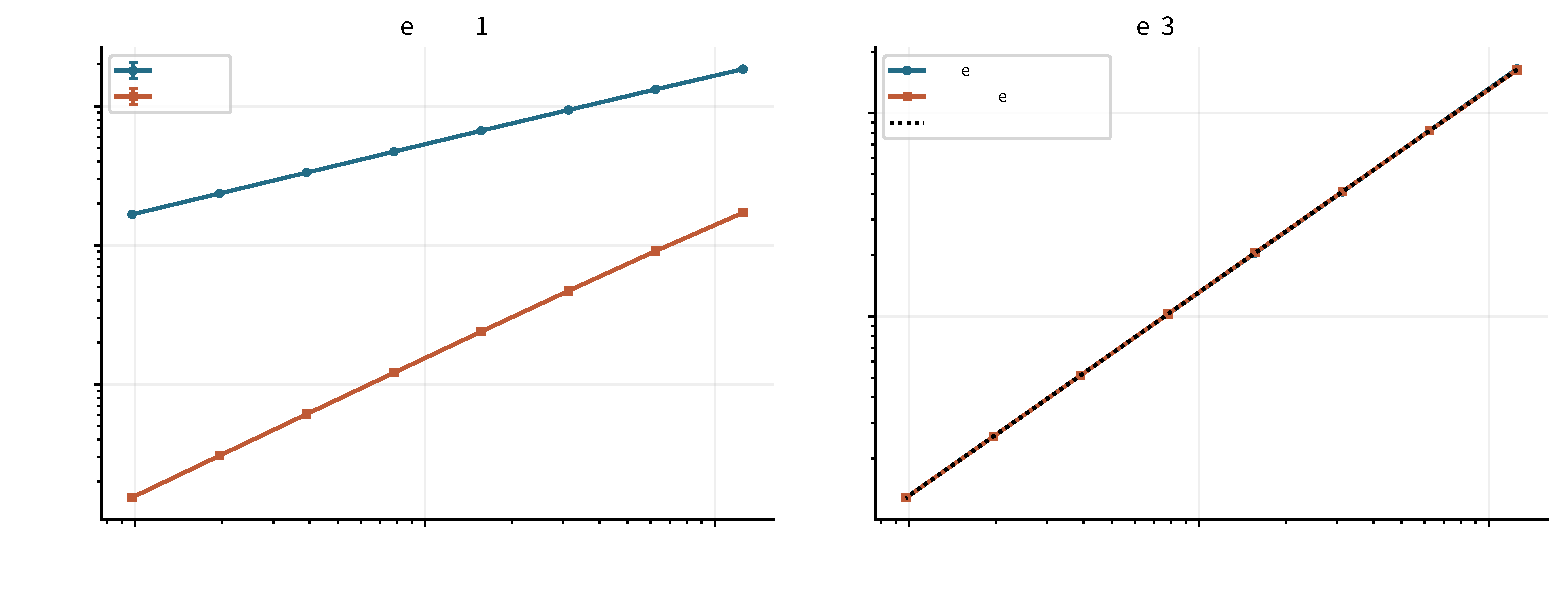
\includegraphics[width=\textwidth]{assets/gbm_results_zh.pdf}
\caption{由现有 CSV 重绘的 GBM 收敛图。左图的误差棒是逐点 95\% 采样区间；右图的三个趋势几乎重合，其精细差异需要结合数值表与区间阅读。}\label{fig:results-gbm}
\end{figure}
图~\ref{fig:results-gbm} 左图的纵轴跨多个数量级，便于看斜率。
斜率接近理论值是算法和实验设计正确的证据，但一张有限样本图不能代替一般收敛定理的证明。

\begin{figure}[htbp]\centering
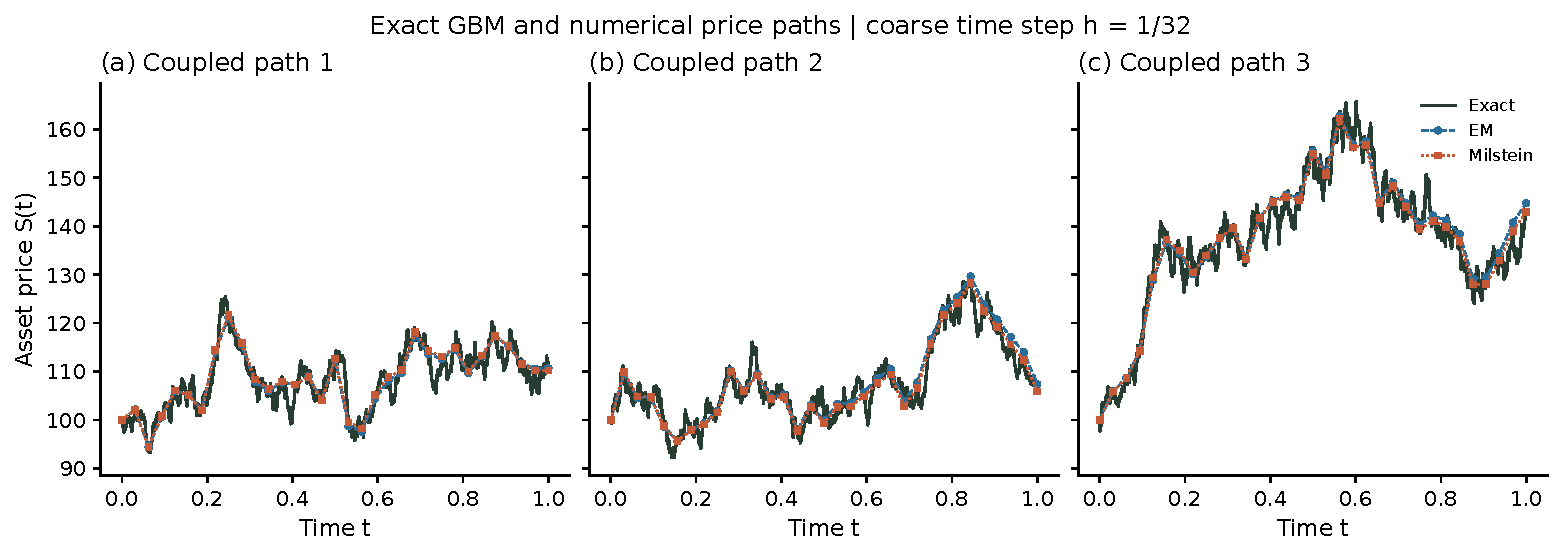
\includegraphics[width=\textwidth]{assets/gbm_paths.pdf}
\caption{原项目的三条共同驱动 GBM 示例路径。Exact 表示精确网格值，EM 与 Milstein 表示价格离散法；粗步长为 $1/32$。横轴是时间，纵轴是价格。}\label{fig:results-paths}
\end{figure}
图~\ref{fig:results-paths} 适合建立“沿同一随机路径逼近”的直觉。
三条样本路径不足以估计收敛阶，而且示例图使用独立于正式实验的随机种子；正式结论来自表~\ref{tab:results-gbm-strong} 的大规模统计。

\subsection{GBM 弱偏差：两种方法为什么几乎一样？}
表~\ref{tab:results-gbm-weak} 将实际控制后估计和解析偏差并列。
两种方法理论均值相同，故该观测量的真偏差相同；模拟值的末位差异来自残余抽样波动。
\begin{table}[htbp]\centering\small
\caption{GBM 的有符号均值偏差：数值减精确。控制后结果仍是模拟估计，解析列是独立核对目标。}\label{tab:results-gbm-weak}
\begin{tabular}{rrrr}\toprule
$N$ & 解析偏差（两方法） & EM 控制后估计 & Milstein 控制后估计\\\midrule
8 & -0.01635672 & -0.01649334 & -0.01629237\\
16 & -0.00819567 & -0.00821180 & -0.00818854\\
32 & -0.00410218 & -0.00409560 & -0.00410591\\
64 & -0.00205218 & -0.00204654 & -0.00205508\\
128 & -0.00102636 & -0.00102512 & -0.00102700\\
256 & -0.00051325 & -0.00051336 & -0.00051318\\
512 & -0.00025664 & -0.00025671 & -0.00025659\\
1024 & -0.00012832 & -0.00012836 & -0.00012831\\
\bottomrule
\end{tabular}
\end{table}

控制后的主窗口斜率分别约为 $0.99874039$ 和 $1.00039041$；解析偏差在全部八个网格上的拟合斜率为 $0.99926631$。
解析曲线并非在所有有限步长上严格等于 $Ch$，还有高阶项，因此有限窗口斜率不必恰好为 1。

最细网格给出一个特别清楚的统计例子：EM 解析偏差为 $-0.0001283247$，
控制后估计为 $-0.0001283595$，95\% 区间为约
$[-0.0001285244,-0.0001281946]$，包含解析目标。
未经控制的配对 EM 区间却跨过零，甚至点估计符号为正。
改善的是估计精度，而不是把 EM 更新公式改成了另一种算法。
Milstein 在最细网格的原始配对区间已经不含零，不能笼统认为所有未经控制的估计都无法分辨偏差。

\subsection{分布图：精确模拟也会与理论曲线有差别}
表~\ref{tab:results-quantiles} 给出 $h=1/8$ 时的分位数；这里用较粗网格使离散差异更容易观察。
\begin{table}[htbp]\centering\small
\caption{GBM 在粗网格 $h=1/8$ 上的分位数。精确模拟列也具有有限样本波动。}\label{tab:results-quantiles}
\begin{tabular}{rrrrr}\toprule
概率 $p$ & 理论分位数 & 精确模拟 & EM & Milstein\\\midrule
0.001 & 39.770 & 39.916 & 37.544 & 40.302\\
0.01 & 50.012 & 49.928 & 48.387 & 50.213\\
0.05 & 61.357 & 61.378 & 60.512 & 61.615\\
0.25 & 82.091 & 82.151 & 82.303 & 82.263\\
0.5 & 100.501 & 100.557 & 101.088 & 100.582\\
0.75 & 123.041 & 123.164 & 123.653 & 123.057\\
0.95 & 164.618 & 164.485 & 163.370 & 164.043\\
0.99 & 201.961 & 202.402 & 198.376 & 201.539\\
0.999 & 253.976 & 256.942 & 247.089 & 255.780\\
\bottomrule
\end{tabular}
\end{table}

例如理论 $1\%$ 分位数约为 $50.012$，EM 为 $48.387$，Milstein 为 $50.213$。
理论 $99\%$ 分位数约为 $201.961$，EM 为 $198.376$，Milstein 为 $201.539$。
这展示了均值以外的分布特征；不同位置不保证每次都按同样顺序接近理论值。

\begin{figure}[htbp]\centering
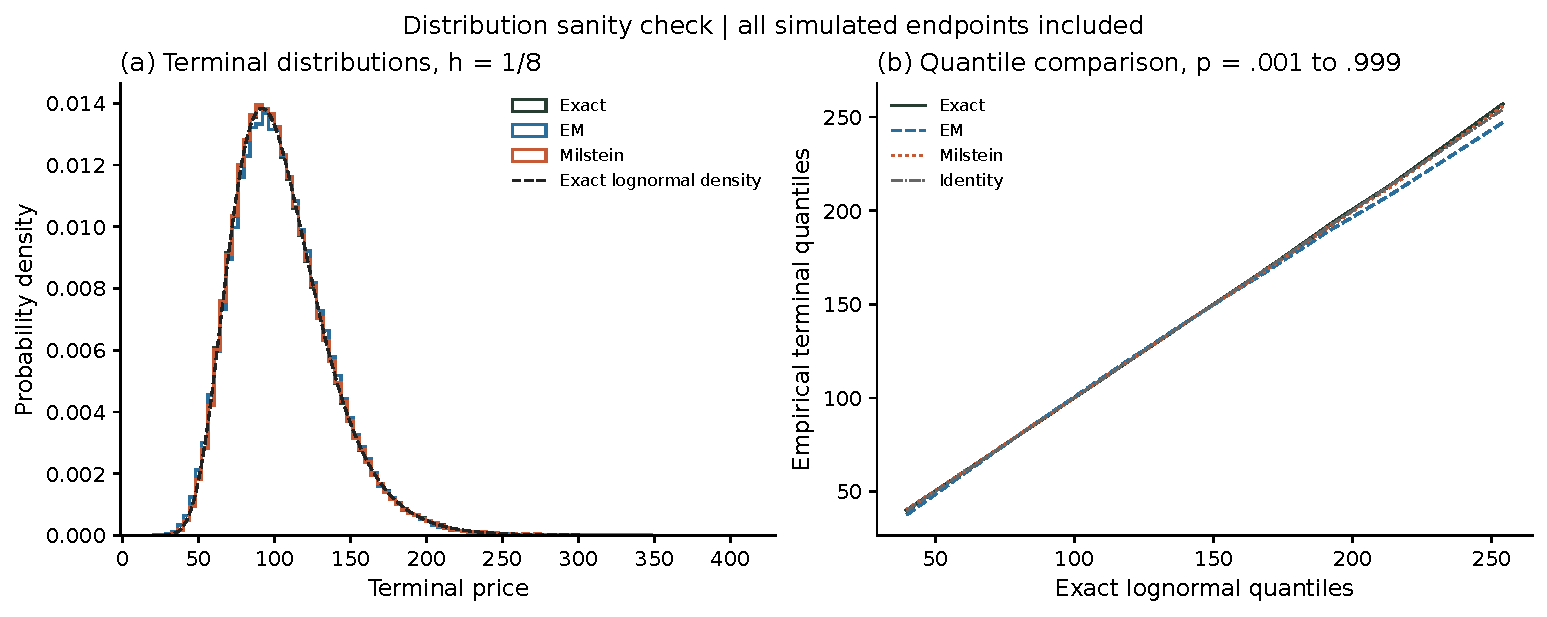
\includegraphics[width=\textwidth]{assets/gbm_distribution.pdf}
\caption{原项目的终值分布图。左图横轴为终值价格，纵轴为密度；右图横轴为理论对数正态分位数，纵轴为经验分位数。Identity 是两者完全相等的参考线。}\label{fig:results-distribution}
\end{figure}
图~\ref{fig:results-distribution} 中即使 Exact 曲线也不会与理论曲线处处重合，因为它来自有限个精确样本。
尾部更容易有较大的采样波动。例如 $0.1\%$ 尾部在 $160000$ 条路径中只有约 $160$ 个观测，极端分位数自然不如中位数稳定。
不能把精确样本与理论分位数之间的每一点差都归咎于时间离散。

\subsection{非仿射强差与弱差：哪些结论已得到支持？}
表~\ref{tab:results-na} 的参考统一为 $8192$ 步。
主强阶窗口是 $N=8,16,32,64$，斜率约为 $0.49145004$。
它支持“该窗口内表现与半阶相容”的判断；由于参考是数值解，应称\emph{经验强阶}。
\begin{table}[htbp]\centering\small
\caption{非仿射模型相对 8192 步参考的结果。100000 条共同路径；区间只量化配对弱差的抽样不确定性。}\label{tab:results-na}
\begin{tabular}{rrrr}\toprule
粗步数 $N$ & 终值强差 & 有符号收益差 & 收益差 95\% 区间\\\midrule
8 & 1.253542 & 0.025793 & $[0.016721,\ 0.034864]$\\
16 & 0.900872 & 0.010477 & $[0.004046,\ 0.016908]$\\
32 & 0.638177 & 0.005402 & $[0.000891,\ 0.009914]$\\
64 & 0.451761 & 0.001722 & $[-0.001479,\ 0.004923]$\\
128 & 0.318537 & 0.000959 & $[-0.001302,\ 0.003220]$\\
256 & 0.223226 & 0.000339 & $[-0.001243,\ 0.001922]$\\
\bottomrule
\end{tabular}
\end{table}


\begin{figure}[htbp]\centering
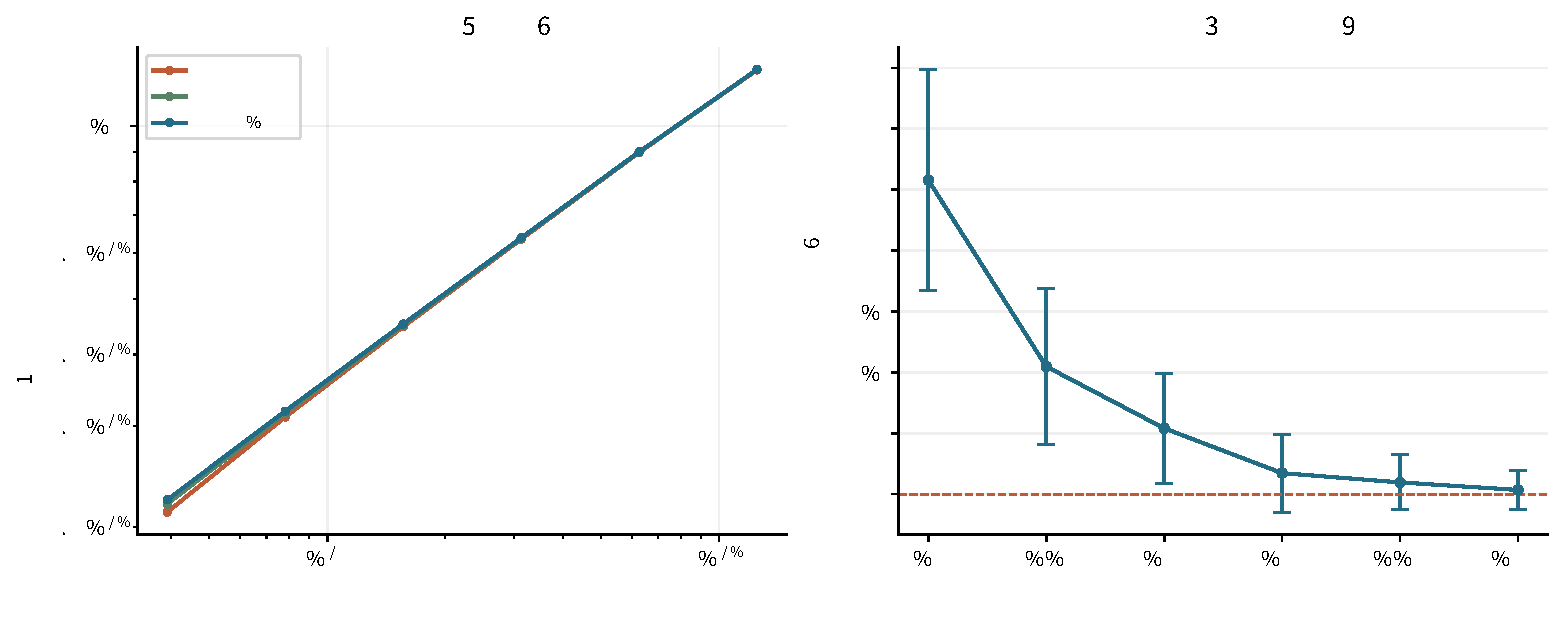
\includegraphics[width=\textwidth]{assets/nonaffine_results_zh.pdf}
\caption{现有非仿射结果的中文重绘。左图比较三层参考；右图保留收益偏差符号及采样区间，能直接看到后三个粗网格的区间跨过零。}\label{fig:results-na}
\end{figure}
图~\ref{fig:results-na} 左图的三条曲线很接近，但更细粗网格处参考影响的\emph{相对}比例增大。
右图前三个点的收益差为正，区间不含零；从 $N=64$ 起区间跨零。
因此当前数据能看到若干粗网格存在可分辨的收益差，却不足以在整个区间上宣称弱一阶。
这不是“实验失败”，而是统计实验对可支持结论作出的边界判断。

最细参考的价格均值为 $105.08796$。其 95\% 区间是 $[104.89962,105.27629]$，包含理论均值 $105.12711$。
但按式~\eqref{eq:ref-discrete-mean}，所有步长都能在期望上匹配这一均值，因此该检查只能作为有限的实现核对。

\subsection{参考加密与驱动检查：不能省掉的配套证据}
表~\ref{tab:results-reference} 显示两个相邻参考差。
收益差很小、区间跨零，说明当前样本没有明显分辨它的符号；强差则仍明显非零。
“收益均值几乎一致”和“同路径终值仍有差异”可以同时成立。
\begin{table}[htbp]\centering\small
\caption{相邻参考网格之间的差。收益差按较粗参考减较细参考计算。}\label{tab:results-reference}
\begin{tabular}{lrrr}\toprule
参考步数加密 & 平均绝对差 & 收益均值差 & 收益差 95\% 区间\\\midrule
2048$\to$4096 & 0.05679005 & -0.00002289 & $[-0.0004228,\ 0.0003770]$\\
4096$\to$8192 & 0.04015705 & 0.00009423 & $[-0.0001879,\ 0.0003763]$\\
\bottomrule
\end{tabular}
\end{table}


非仿射程序在事先指定的第一个批次检验布朗增量，共 $8192\times512=4194304$ 对。
每个增量方差的目标是 $1/8192=0.0001220703125$，实测约为 $0.00012207933$ 与 $0.00012208819$；
实测相关系数约为 $-0.69967521$，目标是 $-0.7$。
这是生成数据后的样本检查，不能只把公式写对就宣称数据诊断已经做过。
它使用第一批增量，并非全部 $100000$ 条路径的所有增量。

状态检查遍历全部网格更新：总更新次数为 $1484000000$。
最细网格保存的 $X$ 极值约为 $2.9739$ 与 $5.6969$，$Y$ 极值约为 $-2.8304$ 与 $1.8819$。
这些 $Y$ 的负值合法；程序报告所有中间 $X,Y$ 有限，并通过指数范围检查。

\subsection{本次独立复核覆盖了什么？}
新增 \texttt{audit\_saved\_results.py} 直接读取原 NPZ、CSV、JSON，独立重算可从终值恢复的统计量。
输出 \texttt{validation\_saved.json} 为 PASS。
它核对 GBM 保存的粗细层强误差、原始配对均值差、分位数和矩公式，以及非仿射的全部 18 组粗参考比较、2 组参考加密、9 层终值与收益统计和强阶拟合。

原保存文件没有储存全部布朗增量和正式控制变量，所以仅靠终值数组无法独立重算控制后的 GBM 弱偏差，也无法重算历史的中间状态检查。
这些部分分别依靠公式与代码审读，以及原运行保存的诊断记录。
本次没有直接运行依赖 Numba 的原 \texttt{verify.py} 内核检查，也没有重新仿真全部大型路径。
教学脚本的确定性检查与小规模运行已单独通过；它们是另一层实现核对，不能冒称重跑了原实验。


\section{按这个顺序亲手练习，并检查自己是否真正理解}\label{sec:practice}
\subsection{四次短练习}
\begin{enumerate}
\item \textbf{只生成布朗运动。} 生成 $N=256$ 个独立 $\sqrt{1/256}Z$，用累计和画路径。
重复许多次，检查 $W_1$ 的样本均值接近 0、方差接近 1。
然后把增量误改为 $(1/256)Z$，亲眼观察累计方差缩小。这能检验你是否理解 $h$ 与 $\sqrt h$。
\item \textbf{只做 GBM。} 固定一批细增量，分别计算精确值、EM、Milstein。
先手算一条路径的一个时间步，再对应代码。把细增量求和成粗增量，比较终值强误差。
使用 \texttt{teaching\_demo.py} 的默认输出，不急着拟合精细弱阶。
\item \textbf{再加非仿射模型。} 先把 $g_{\min}=g_{\max}=0.3$，此时资产部分退化为常波动率 GBM，对数 EM 应在每个网格精确。
恢复原来的 $0.1,0.5$ 后，再看参考网格差。
这个退化测试能同时发现 Itô 补偿项、粗化和旧状态更新方面的错误。
\item \textbf{最后学习统计精度。} 比较原始弱偏差和控制后弱偏差的标准误差；
再阅读原大样本的 CSV。尝试解释为什么“点估计更接近零”本身不能证明方法阶数更高。
\end{enumerate}

\subsection{常见错误清单：每一项都对应一种具体后果}
\begin{table}[htbp]\centering\small
\caption{代码与理论中最常见的混淆。}\label{tab:practice-errors}
\begin{tabularx}{\textwidth}{YY}\toprule
错误操作或判断 & 为什么会出问题\\\midrule
用 $hZ$ 代替 $\sqrt h Z$ & 累计噪声方差随网格加密消失\\
给每个时刻独立抽取 $N(0,t)$ & 边际正确、时间联合关系错误\\
对 $\log S$ 使用普通链式法则 & 漏掉 $-\sigma^2/2$，价格均值出错\\
粗细网格分别抽独立噪声 & 强差包含不同随机路径的天然差异\\
把 $\E|D|$ 当成弱偏差 & 正负误差无法抵消，计算了另一种量\\
把标准差当成均值标准误差 & 忘记除以 $\sqrt M$，误读统计精度\\
弱偏差区间跨零后继续强行拟合 & 容易测出噪声造成的虚假斜率\\
先更新 $Y$，再用新 $Y$ 更新 $X$ & 破坏既定的同步左端 EM\\
认为 $Y<0$ 就是负波动率 & 实际波动率是始终为正的 $g(Y)$\\
把三层参考看作三份精确解 & 忽略所有参考仍有时间离散偏差\\
把平均收益直接称为期权价格 & 缺少定价测度与贴现设定\\
只保存随机种子就保证逐位复现 & 批大小、数组布局、版本等也影响随机数分配和浮点结果\\\bottomrule
\end{tabularx}
\end{table}
表~\ref{tab:practice-errors} 可以作为读代码时的自查表；理解每一行的原因，比背下一张方法阶数表更重要。

\subsection{自测与参考答案}
\begin{enumerate}
\item \textbf{步长从 $1/64$ 改成 $1/256$，EM 强半阶意味着误差大约缩小几倍？}
答：步长缩小四倍，误差约缩小两倍。路径数不变时，不能据此断言所有统计量的置信区间也恰好缩小两倍。
\item \textbf{模拟的 GBM 均值不等于 $105.1271$，一定是程序错了吗？}
答：不是。即使精确模拟，有限样本均值也有抽样误差；应比较理论目标与合理的标准误差、置信区间。
若是 EM/Milstein，还存在可解析计算的均值离散偏差。
\item \textbf{为什么 Milstein 强误差更小，但 GBM 均值弱偏差与 EM 相同？}
答：Milstein 加入的二次随机修正改善逐路径逼近；该修正条件期望为零，两种方法的一步平均乘子仍都是 $1+\mu h$。
\item \textbf{把非仿射参考从 4096 步增加到 8192 步，差异很小，是否已证明真误差很小？}
答：没有。它检验了对参考加密的敏感性；若无额外理论界，无法把参考差等同于参考真误差。
\item \textbf{为什么非仿射模型的粗网格价格均值也能正确？}
答：冻结 $g(Y_n)$ 后，指数正态的条件期望恰好抵消 $-g_n^2h/2$。
均值精确保留，但路径与非线性收益不一定准确。
\item \textbf{控制变量是不是利用已知答案“作弊”？}
答：不是。控制量的均值已知为零，独立预实验拟合后，减去它不会改变目标期望。
解析偏差只作为核对列；正式估计仍由新的随机样本计算。
\item \textbf{非仿射两维噪声相关，为什么下一步仍能对当前状态条件取期望？}
答：两个未来增量彼此可以相关，但整对未来增量与过去信息独立。
当前 $Y_n$ 已知，不等于未来 $Y_{n+1}$ 已知。
\item \textbf{精确转移是否表示画出的折线就是连续真解？}
答：不是。精确的是所选网格时刻的值及其联合分布。两点之间画直线只是一种展示方式，并未模拟出全部布朗桥波动。
\end{enumerate}

\subsection{如果需要用自己的话说明整份项目}
可以按以下逻辑组织一次口头讲解：价格存在连续累积的随机冲击，所以用布朗运动驱动的 SDE；
Itô 公式说明为何对数变换产生二阶补偿项，由此得到 GBM 的精确基准；
EM 冻结一步系数，Milstein 加入噪声强度变化造成的二阶项；
强误差检验同路径逼近，弱误差检验观测函数的期望，二者都需要与有限样本噪声区分；
最后，把共同增量、参考加密与置信区间用于没有精确采样器的非仿射模型。
每一步都应能指向一条公式、一段代码或一份保存的统计证据。

\section{材料来源、文件使用与进一步阅读}\label{sec:sources}
本讲义依据用户提供的 \texttt{problem\_pack.pdf} 第 6--7 页，以及当前文件夹中的
\nolinkurl{Problem4_FinancialSDE_Coursework.tex}、\texttt{gbm.py}、\texttt{nonaffine.py}、
\texttt{verify.py}、\texttt{build\_report\_data.py}、\texttt{run\_all.py} 和保存结果编写。
下载目录中的原题 PDF 与项目 \texttt{source/problem\_pack.pdf} 经 SHA-256 比较完全一致。
原题里的任务要求在此作为讲解对象；这份学习讲义按用户的中文教学请求编写，不受原英文报告 12 页篇幅限制。

本次新增的主文件是 \texttt{Problem4\_Chinese\_Tutorial.tex} 和同名 PDF，位于 \texttt{tutorial\_zh/}。
TeX 主文件已经合并章节和数值表，编译时只需同目录的 \texttt{assets/} 图文件与所需字体、宏包；
\texttt{drafts/} 是制作时的章节片段，阅读或重新编译主文件不依赖它。
\texttt{build\_assets.py} 从原保存数据重绘中文图表；\texttt{teaching\_demo.py} 运行教学示例；
\texttt{audit\_saved\_results.py} 复核保存统计。
原大型实验的输出文件没有被本讲义的教学程序覆盖。

在此目录运行以下任一方式可编译：
\begin{lstlisting}[language={}]
tectonic --keep-logs Problem4_Chinese_Tutorial.tex

# Or, with a full TeX distribution:
xelatex -interaction=nonstopmode -halt-on-error Problem4_Chinese_Tutorial.tex
xelatex -interaction=nonstopmode -halt-on-error Problem4_Chinese_Tutorial.tex
\end{lstlisting}
中文字体使用 Noto Serif CJK SC、Noto Sans CJK SC 和 Noto Sans Mono CJK SC。
本机以 Tectonic 编译；在其他机器上可安装同名字体，或修改导言区的字体配置。

进一步学习可读 Higham 的算法入门文章\cite{higham}。
它面向具有基础概率知识的读者，用小程序讨论布朗运动、随机积分、EM、Milstein 及强弱收敛。
作者维护的示例程序页面还列出了原文和代码勘误，适合与本题的 Python 实现对照阅读。
本讲义的详细演算围绕用户的具体题目与既有代码重新展开，不要求读者先读完该文。

\noindent\textbf{编写说明。}本讲义由 AI 根据所提供材料进行中文教学组织、数学推导、代码示例编写、保存数据复核与排版生成；未声称经过教师或作者的人工作业评审。

\begin{thebibliography}{9}
\bibitem{pack} 用户提供的 \emph{Problem Pack: Five Suggested Directions for the ODE IVP Project}，Direction 4，第 6--7 页。项目内副本：\texttt{source/problem\_pack.pdf}。
\bibitem{report} 项目已有 \emph{Numerical Simulation of Financial SDEs: Problem 4 GBM Benchmark and Non-Affine Volatility}，2026 年 9 月；配套 Python 源码与 \texttt{results/} 保存结果。
\bibitem{higham} D. J. Higham. An Algorithmic Introduction to Numerical Simulation of Stochastic Differential Equations. \emph{SIAM Review}, 43(3), 525--546, 2001.
\href{https://doi.org/10.1137/S0036144500378302}{doi:10.1137/S0036144500378302}。
\href{https://webhomes.maths.ed.ac.uk/~dhigham/algfiles.html}{作者的示例程序与勘误页面}。
\end{thebibliography}
\end{document}
